\chapter{Experimentos}
\label{experimentos}
A lo largo de esta sección, se tratarán de forma detallada los distintos experimentos que se han realizado para este proyecto con el fin de 
poner en práctica los conocimientos obtenidos durante el proceso de investigación de la materia. Para los experimentos se planteará cuál es el 
objetivo a alcanzar y los posibles enfoques a aplicar para llegar a una solución, además de tratar los retos encontrados por el camino, los 
resultados del experimento y las lecciones que puedan ser aprendidas de este.

\section{Introducción al uso de Qiling: Prueba de concepto y fuzzing}
\subsection{Introducción al experimento}
En la sección de ''\nameref{estado_del_arte}'' decíamos que hay ciertos casos para los que no nos interesa fuzzear la ejecución de principio a fin 
de un programa como cuando hacemos frente a un software complejo y costoso en tiempo de ejecutar o cuando para llevar a cabo la ejecución correctamente, 
necesitamos de algún periférico o recurso del que carecemos. Además, la idea de poder dirigir el proceso de fuzzing a los componentes del código que más nos 
resulten de interés es de alto valor para nuestro principal objetivo al realizar fuzzing, la identificación de vulnerabilidades en el menor tiempo posible.
Emuladores como Unicorn o Qiling hacen esto posible gracias a sus capacidades no solo de emulación sino también de instrumentación dinámica de binarios.
Cuando se decidió poner en práctica esta técnica para realizar fuzzing orientado a IoT, fue necesario elegir entre estos dos proyectos, los cuales 
representan a día de hoy los principales emuladores multi-arquitectura centrados en la instrumentación dinámica a través de una API. Qiling terminó siendo 
la elección final gracias a que además de presentar toda la funcionalidad de Unicorn, nos permite trabajar a más alto nivel con conceptos como librerías dinámicas,
llamadas al sistema o I/O, al contrario que este otro que solo trabaja a nivel de instrucciones de CPU.\bigskip

El objetivo de este pseudo-experimento es servir de una breve toma de contacto práctica con las capacidades del framework de Qiling, para facilitar la comprensión 
del siguiente experimento a realizar, donde usaremos Qiling entre otras herramientas para analizar una vulnerabilidad real recientemente descubierta en un router
inteligente. Llevar a cabo esta toma de contacto inicial resulta de gran ayuda ya que aunque el código que vamos a emular y fuzzear a continuación 
no pertenece a un caso real, puede resultar abrumador intentar introducirnos directamente en el mundo de la instrumentación dinámica sobre binarios encontrados en 
imágenes firmware de dispositivos IoT reales debido a su complejidad. Por ello,empezaremos instrumentando un simple ejemplo de código creado por nosotros mismos que 
buscará simular comportamientos problemáticos comúnmente encontrados al realizar fuzzing de binarios de dispositivos empotrados/IoT reales.\bigskip

Más concretamente, este pseudo-experimento a modo de prueba de concepto consistirá en la emulación y fuzzing mediante Qiling de un simple binario que tras 
dormir durante cinco segundos lleva a cabo el ''cifrado'' de un string introducido como parámetro mediante la aplicación de una operación
XOR a cada byte del string. El tiempo durante el cual el binario duerme intenta simbolizar escenarios problemáticos reales de cara al fuzzing 
como la ejecución de rutinas de código previas a la funcionalidad que queremos evaluar o el bloqueo temporal de la ejecución por ocasionados 
por no conseguir emular el entorno de ejecución real a la perfección. En cualquiera de los casos, este tipo de comportamientos dificulta
enormemente el obtener buenos resultados a través del fuzzing como probaremos a continuación.

\subsection{Realización del experimento}
Empezaremos por desarrollar un simple código en C que implemente la funcionalidad descrita anteriormente. Además, añadiremos a la función de 
cifrado de strings un crash forzado por una lectura de array fuera de límites que se dará cuando el string introducido empiece por el carácter
'a' y tenga una longitud mayor que diez caracteres. Esto nos servirá para evaluar la efectividad de nuestra solución de fuzzing para dar con 
el input que origina este crash. El código mostrado a continuación será compilado para ARM, que como ya sabemos se trata de una arquitectura 
comúnmente encontrada en dispositivos IoT y lo haremos usando compilación cruzada con el toolchain de GNU para ARM.

\begin{lstlisting}[language=C, caption=Código de ejemplo a fuzzear., captionpos=b,
    frame=single, breaklines, showstringspaces=false]
    #include <stdio.h>
    #include <unistd.h>
    #include <string.h>
    #include <stdlib.h>

    void printRes(char str[], unsigned len){
        printf("Ciphered output: ");
        for (unsigned i = 0; i < len; ++i)
            printf("\\x%02X", str[i]);
        printf("\n");
    }

    void processArgs(char str[]){
        unsigned len = strlen(str);
        
        if (len > 10 && str[0] == 'a'){
            printf("CRASH");
            char dst[2];
            dst[6] = str[0];
        }

        for (unsigned i = 0; i < len; ++i){
            str[i] = (char)(str[i] ^ 'c');
        }

        printRes(str, len);
    }

    int main(int argc, char* argv[]){
        if (argc != 2){
            printf("Usage: %s <input_string>\n", argv[0]);
            exit(1);
        }
        
        sleep(5);
        processArgs(argv[1]);
    }
\end{lstlisting}

\subsubsection{Intento de fuzzing mediante AFL++ en modo QEMU}
Con el fin de ejemplificar como un comportamiento como este puede resultar desastroso de cara a fuzzear un binario, intentamos fuzzear el 
código mostrado mediante técnicas más tradicionales como puede ser el uso de AFL++ en su modo QEMU (emulación user-mode). Este modo de AFL++ es el 
modo por defecto recomendado cuando se desea hacer fuzzing sobre un binario que no ha sido instrumentado. Para ello, preparamos un input 
básico con la cadena ''BBBBBB'' e iniciamos el fuzzing (figura \ref{fig:QEMUPoC}) con la siguiente orden (Fijamos la variable de entorno
''QEMU\_LD\_PREFIX'' a la ruta que contiene las librerías necesarias en tiempo de ejecución, -Q indica a AFL++ que ha de usarse el modo QEMU y
-t el valor del timeout en milisegundos el cual deberá ser mayor que el valor utilizado en la llamada a \textit{sleep}):

\begin{lstlisting}[language=bash]
    $ QEMU_LD_PREFIX=/usr/arm-linux-gnueabi afl-fuzz -i fuzz_setup/in -o fuzz_setup/out -Q -t 7000 -- ./bin/main_arm @@
\end{lstlisting}

\begin{figure}[H]
    \centering
    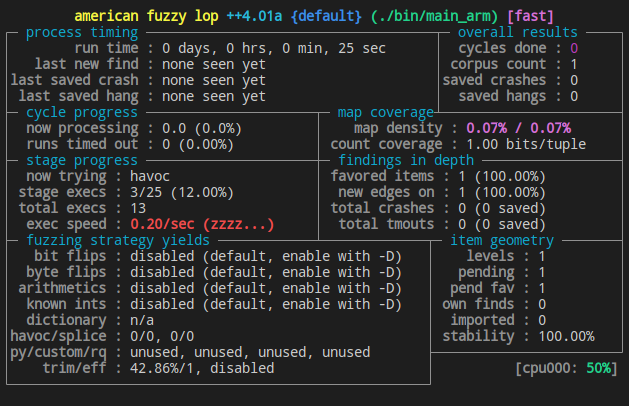
\includegraphics[scale=0.59]{QEMUPoC.png}
    \caption{AFL++ fuzzeando código problemático en modo QEMU.}
    \label{fig:QEMUPoC}
\end{figure}

Observando la información reportada por AFL++, salta a la vista que el número de ejecuciones por segundo es demasiado bajo como para encontrar 
el crash que buscamos en un tiempo razonable.

\subsubsection{Uso de Qiling}
Qiling proporciona funciones en su API para llevar a cabo diversas tareas de instrumentación dinámica que pueden sernos de utilidad en este 
tipo de casos en los que métodos más tradicionales de fuzzing pueden no ser viables. Ejemplos de funcionalidades interesantes son los snapshots,
que pueden acelerar el fuzzing guardando el estado de la CPU y la memoria en un momento dado y restaurarlo para cada iteración, las operaciones 
con memoria y registros, que nos permiten trabajar con los parámetros de las funciones, los hooks, que hacen posible ejecutar código propio al 
llegar a una dirección del programa específica o el mapeo de dispositivos del host al entorno de emulación. De todo esto haremos uso de las 
operaciones con memoria y registros de la CPU para modificar el punto de entrada del binario a la función de cifrado que deseamos fuzzear e 
instrumentarla, además de usar hooks para automáticamente realizar dichas operaciones al alcanzar puntos estratégicos del binario durante la 
ejecución.\bigskip

Dado que estamos ante un binario simple, su emulación con Qiling no requiere de ninguna instrumentación adicional. Para emular el binario 
hacemos uso de ''qltool'', la herramienta proporcionada por Qiling para emular rápidamente binarios sin aplicar instrumentación. Utilizamos la 
siguiente orden y observamos como el binario compilado para ARM se ejecuta correctamente, mostrando tras cinco segundos de espera los
bytes de la cadena resultante en hexadecimal (figura \ref{fig:qltool}).

\begin{lstlisting}[language=bash]
    $ qltool run --rootfs /usr/arm-linux-gnueabi -f bin/main_arm --args abc
\end{lstlisting}

\begin{figure}[H]
    \centering
    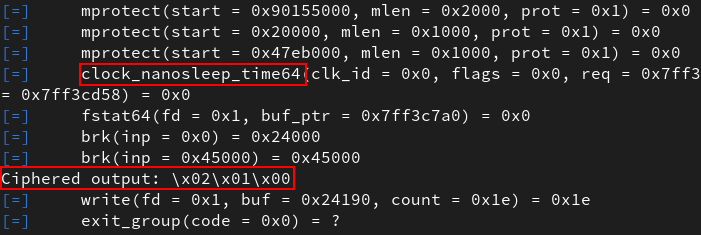
\includegraphics[scale=0.59]{qltool.png}
    \caption{Emulación de código ARM con qltool.}
    \label{fig:qltool}
\end{figure}

Ahora, para aplicar fuzzing consiguiendo buenos resultados necesitaremos hacer uso de instrumentación dinámica que nos permita saltar esa pausa que 
simula una sección de código problemática. Para esto, crearemos un script de Python en el que haremos uso de la API de Qiling para modificar
el flujo de ejecución del binario y usar como ''main'' del programa la función de cifrado de cadenas de texto. Como fuzzer a utilizar junto a Qiling, 
haremos uso de AFL++ gracias a su fácil integración con Unicorn y Qiling a través de Unicornafl lo cual nos permitirá realizar fuzzing aprovechando la 
información de cobertura de código proporcionada por Qiling. Además, ya que durante el fuzzing 
no nos interesa que la cadena resultante se muestre por pantalla, también podemos finalizar la ejecución en la dirección donde se encuentre la instrucción
de retorno de la función ''processArgs()'', reduciendo así el número de instrucciones a ejecutar. En la figura \ref{fig:QilingFuzzDiagram} observamos el
flujo de ejecución que se desea llevar a cabo para fuzzear el código.

\begin{figure}[H]
    \centering
    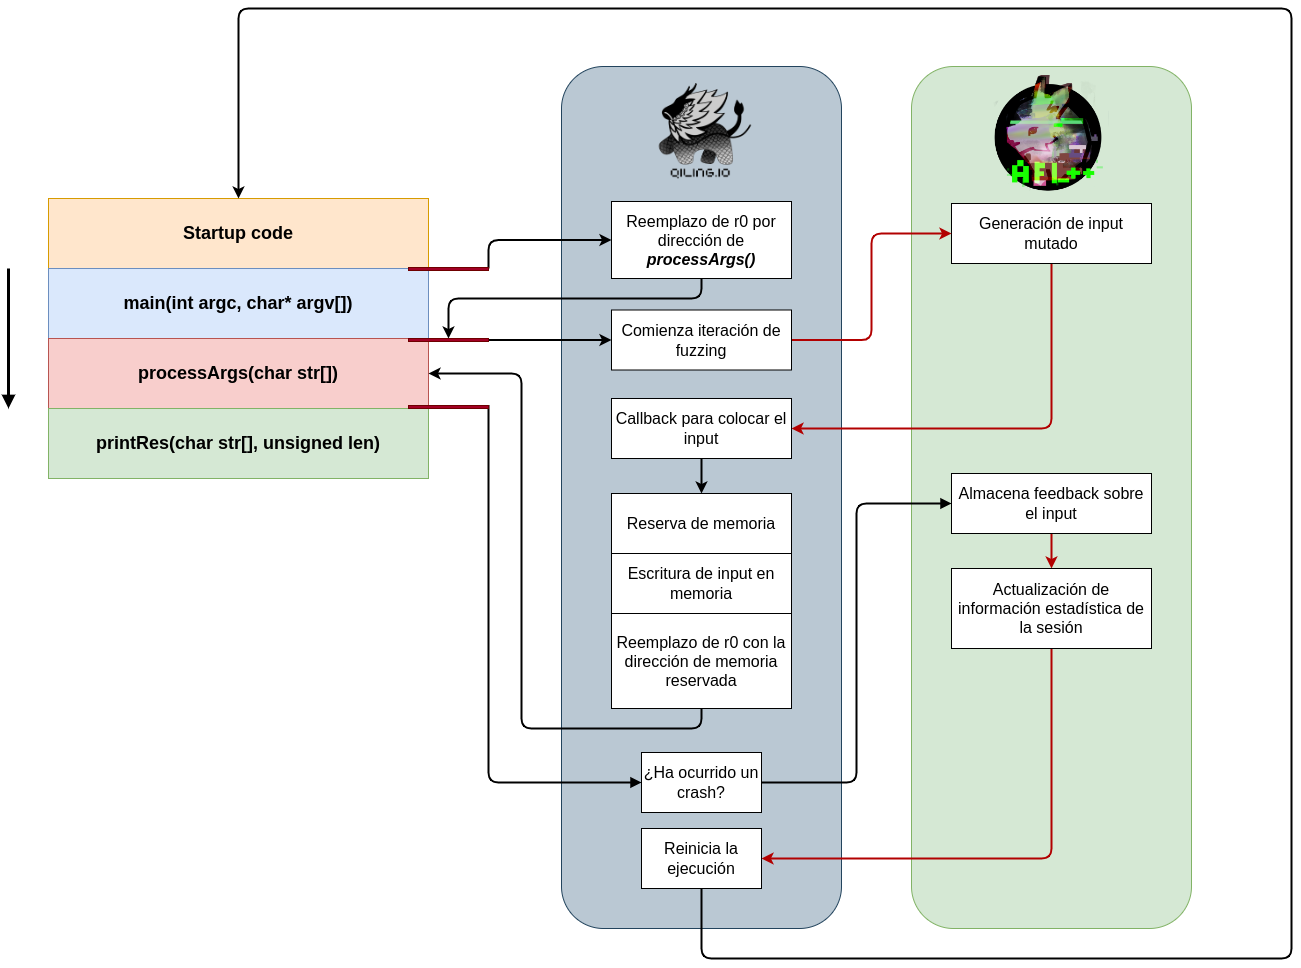
\includegraphics[scale=0.26]{QilingFuzzDiagram.png}
    \caption{Diagrama simplificado del proceso de fuzzing a implementar en Qiling.}
    \label{fig:QilingFuzzDiagram}
\end{figure}

Para llevar a cabo el diagrama mostrado, empezamos estableciendo el hook y el callback que cambie el punto de entrada de ''main()'' por ''processArgs()''.
La API de Qiling ofrece la función ''hook\_address(callback, trigger\_address)'' que toma como parámetros la función de Python a llamar a modo de callback 
y la dirección de una instrucción dentro del binario para la cual llamar al callback previamente a su ejecución. La dirección elegida para fijar el callback 
será la de la llamada a ''\_\_libc\_start\_main()'' como parte del proceso de setup realizado por el binario previamente a ejecutar su main. El callback
simplemente usará la función ''ql.arch.regs.write(register\_id, value)'' de la API de registros de CPU de Qiling para fijar el valor del registro R0 a la dirección de la primera 
instrucción de ''processArgs()''. Lo que se consigue modificando R0 es alterar el primer parámetro de la llamada a una función en ARM32. Aplicamos esta
técnica en lugar de fijar directamente el contador de programa a la primera instrucción de ''processArgs()'' para conservar el código 
de inicialización del entorno de ejecución y evitar así diversos problemas como errores de enlazado de librerías dinámicas.\bigskip

Por último, integramos la ejecución de la función con AFL++ mediante un hook adicional que inicie la iteración de fuzzing y un callback que pueda ser 
llamado por AFL++ para introducir el input mutado en memoria. En el snippet de código mostrado a continuación vemos también como el callback ha de 
reservar y escribir en memoria los bytes del input ya que la función a fuzzear utiliza un string como parámetro.

\begin{lstlisting}[language=python, caption=Integración de AFL++ con nuestro script de Qiling., captionpos=b,
    frame=single, breaklines]
    ...
    def place_input_callback(_ql: Qiling, input: bytes, _):
        address = _ql.mem.map_anywhere(len(input))
        _ql.mem.write(address, input)
        _ql.arch.regs.write("r0", address)

    def start_afl(_ql: Qiling):
        ql_afl_fuzz(_ql, param_file, place_input_callback, exits=[ql.os.exit_point])

    ql.hook_address(start_afl, TARGET_FUNC_ADDR)

    ...
\end{lstlisting}

Para comenzar la sesión de fuzzing utilizamos como input inicial un fichero con la cadena ''BBBBBB'' y utilizamos la siguiente orden para 
indicar a AFL++ que utilice nuestro script en modo Unicorn (figura \ref{fig:QilingPoCfuzz}). 

\begin{lstlisting}[language=bash]
    $ afl-fuzz -i fuzz_setup/in -o fuzz_setup/out -U -- python3 src/fuzz.py @@
\end{lstlisting}

\begin{figure}[H]
    \centering
    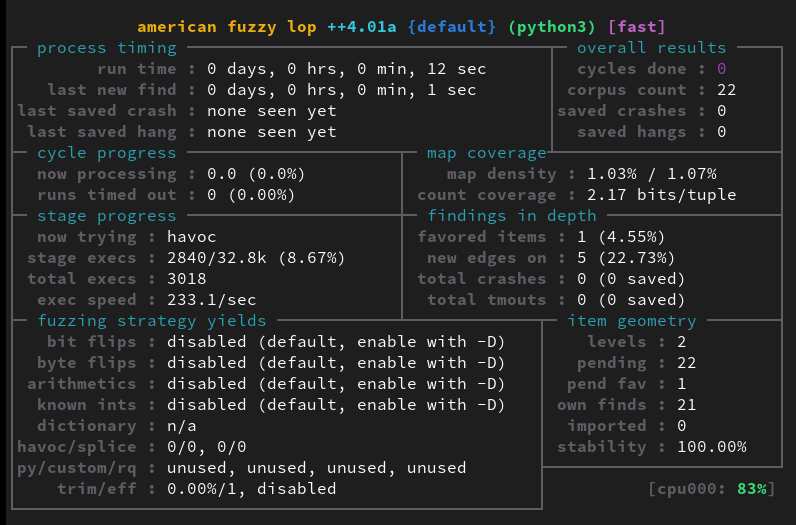
\includegraphics[scale=0.40]{QilingPoCfuzz.png}
    \caption{Prueba de concepto de fuzzing con Qiling y AFL++.}
    \label{fig:QilingPoCfuzz}
\end{figure}

\subsection{Resultados}
Hemos podido comprobar que el fuzzing de nuestro código de prueba utilizando AFL++ en modo QEMU ha resultado ser un fracaso en términos de 
eficiencia, como era de esperar. En cambio,
al aplicar técnicas de instrumentación dinámica en Qiling hemos conseguido una mejora abismal en el número de ejecuciones por segundo durante el fuzzing, 
yendo de menos de una ejecución por segundo en QEMU a alrededor de doscientas con Qiling. Pasando a la detección de la vulnerabilidad introducida, 
cabe mencionar que hubo problemas para registrar correctamente los crashes producidos. Tras un poco de investigación, parece ser que Qiling en su versión developer
(recomendada en la documentación oficial frente a la estable) ha sufrido una regresión en el tratamiento de crashes ya que Qiling estable es capaz de 
reportar a AFL++ cuando nuestro código crashea debido a lectura fuera de límites introducida, mientras que en su versión developer el crash no es reportado.
Tras crear una \href{https://github.com/qilingframework/qiling/issues/1163}{issue} en el repositorio oficial de Qiling\cite{qiling}, el bug ha sido reconocido y está siendo corregido actualmente.


\subsection{Lecciones aprendidas}
A través de la realización de esta pequeña prueba de concepto ha quedado patente el potencial de Qiling cuando se trata de llevar a cabo tareas relacionadas
con la instrumentación dinámica de binarios, como es el fuzzing. Teniendo en cuenta que este ejemplo se trata solo de una pequeña toma de contacto con la herramienta
para introducirnos a su uso, donde realmente aprenderemos sobre casos prácticos reales de aplicación de Qiling es en el experimento a continuación.

\section{Identificación de vulnerabilidad real a través de fuzzing: Netgear R7000}\label{r7000_section}
\subsection{Introducción al dispositivo}
El Netgear R7000, también conocido como Nighthawk AC1900 es un router WIFI ''inteligente'' lanzado al mercado originalmente en 2013 con una última
revisión del hardware en 2018 que sigue en venta actualmente. Este producto de la gama de routers premium de Netgear recibe actualizaciones periódicas
a día de hoy por parte del fabricante y se trata de una elección muy popular entre aquellos consumidores que buscan un router dual-band de altas prestaciones. 
\begin{figure}[H]
    \centering
    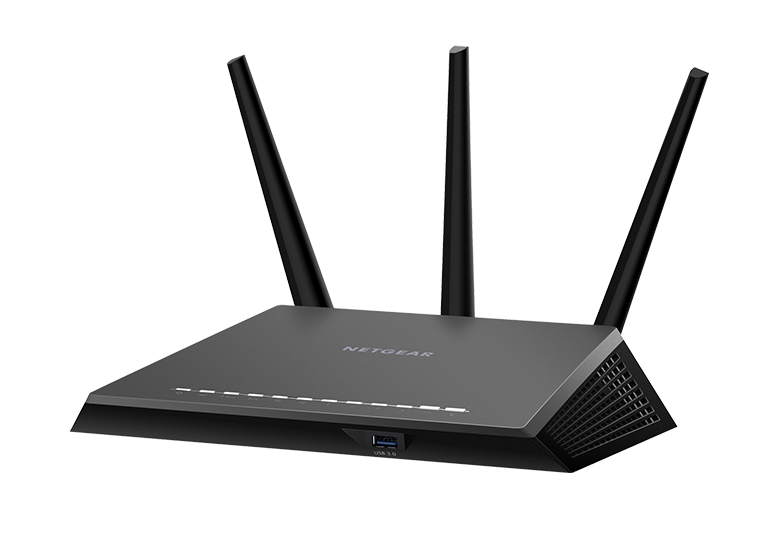
\includegraphics[scale=0.30]{r7000.png}
    \caption{Netgear R7000 (Nighthawk AC1900).}
    \label{fig:r7000}
\end{figure}

\subsection{Recopilación de información}
Consultando sus especificaciones técnicas principales 
encontramos que posee una CPU de 1GHz dual-core, 256MB de RAM, 128MB de memoria flash y soporte para dual-band de 2'4GHz a 600Mbps y de 5GHz a 
1300Mbps. Aunque estas especificaciones son interesantes a la hora de conocer las restricciones cómo de restringido en rendimiento es el dispositivo,
no son lo suficientemente detalladas como para aportarnos información clave que necesitamos conocer para aplicar emulación sobre el dispositivo.
Principalmente, desconocemos el procesador que está siendo utilizado y su arquitectura, ya que el fabricante no proporciona dicha información.
Cuando nos encontramos en esta situación en la que deseamos conocer información más detallada sobre los componentes internos de un dispositivo, 
una posible solución es consultar su informe de aceptación para la certificación del FCC\cite{fcc} en la base de datos \hyperlink{fccid.io}{fccid.io}.
El FCC es un organismo de certificación encargado de evaluar todo producto que vaya a ser comercializado en los Estados Unidos que emita 
radiofrecuencias con el fin de asegurar que dichos dispositivos no produzcan interferencias dañinas que pudieran afectar al correcto
funcionamiento de otros dispositivos como equipamiento médico, aeronáutico o sistemas de telecomunicaciones.\bigskip

Accediendo a la base de datos podemos encontrar información de los reportes que se han ido realizando sobre las distintas iteraciones del producto,
concretamente, el reporte de mayor interés para nuestra tarea es el titulado ''Internal Photos'' publicado para la revisión lanzada en 2018\cite{netgearFCCid}.
Buscando lo que pudiera ser la CPU principal nos llaman la atención dos chips mostrados en el informe. El primero (figura \ref{fig:r7000transceptor}), al 
consultar la ficha técnica del BCM4360 descubrimos que se trata de un transceptor WIFI del fabricante Broadcom, por lo tanto no es lo que tratamos de 
encontrar. Respecto al segundo chip (figura \ref{fig:r7000cpu}), consultando las especificaciones presentes en la ficha técnica del Netgear R7000 
(tabla \ref{table:r7000}) proporcionada por OpenWRT podemos ver que se trata de un System on a Chip (SoC) WIFI lanzado al mercado en 2013\cite{broadcomSOCs} 
que en su interior contiene un procesador dual core ARM Cortex A9 de 32 bits.

\begin{figure}[H]
    \centering
    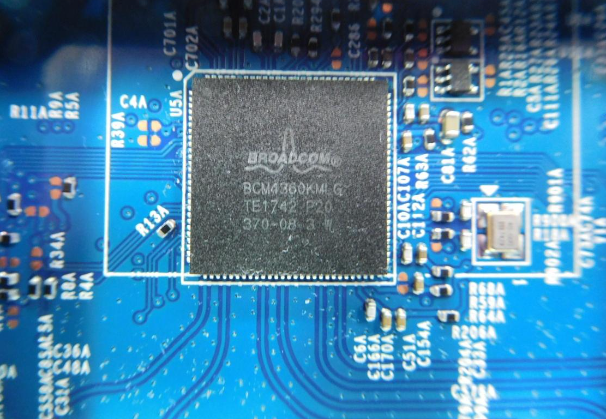
\includegraphics[scale=0.45]{r7000transceptor.png}
    \caption{Broadcom BCM4360 en el interior del Netgear R7000.\cite{netgearFCCid}}
    \label{fig:r7000transceptor}
\end{figure}

\begin{figure}[H]
    \centering
    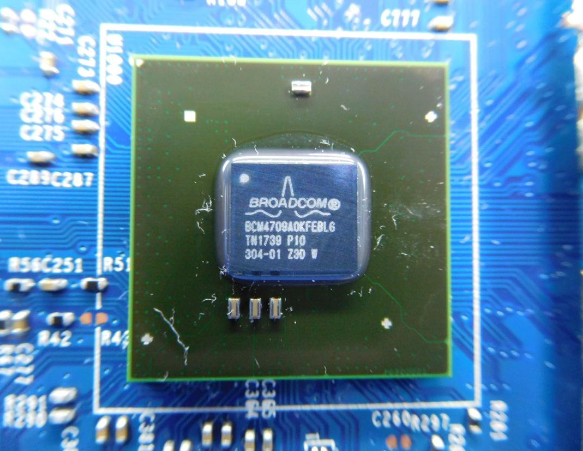
\includegraphics[scale=0.59]{r7000cpu.png}
    \caption{Broadcom BCM47 en el interior del Netgear R7000.\cite{netgearFCCid}}
    \label{fig:r7000cpu}
\end{figure}

\begin{table}[H]
    \centering
    \begin{tabular}{ |l|m{20em}| }
    \hline
    FCC ID                      & PY313200233                      \\\hline
    Industry Canada ID          & 4054A-13200233                   \\\hline
    Voltaje                     & 12 VDC, 3.5 A                    \\\hline
    CPU/SoC                     & Broadcom BCM4709A0 @1 GHz        \\\hline
    Arquitectura CPU            & ARM Cortex A9 (2 cores)          \\\hline
    Flash / RAM                 & 128 MiB / 256 MiB                \\\hline
    Chip WI1 \& WI2             & Broadcom BCM4360                 \\\hline
    Protocolos WI1 \& WI2       & an+ac / bgn                      \\\hline
    Configuración MIMO wireless & 3x3:3                            \\\hline
    Conector de antena          & U.FL, RP-SMA                     \\\hline
    Switch \& Ethernet          & Broadcom BCM4709A0               \\\hline
    Puertos WAN/LAN             & 1 / 4 (up to 1 Gb/s)             \\\hline
    Puertos USB                 & 1x USB 3.0, 1x USB 2.0           \\\hline
    Puerto serie                & 4-pin header, internal, 3.3V TTL \\\hline
    \end{tabular}
    \caption{Especificaciones del Netgear R7000.\cite{r7000datasheet}}
    \label{table:r7000}
\end{table}

Aunque Broadcom no proporciona una datasheet con las especificaciones del SoC, 
si que podemos consultar información más detallada sobre el Cortex A9 a través de la documentación oficial de ARM\cite{cortexA9}. Gracias a esto podemos 
conocer detalles como información sobre la Memory Management Unit (MMU) que utiliza la CPU. Esta información es de gran importancia ya que como explicaban
Muench et al.\cite{Muench2018}, la presencia de una MMU en un dispositivo empotrado puede alterar drásticamente el comportamiento de este ante corrupciones de 
memoria. Un dispositivo sin MMU puede no detectar fallas de memoria y seguir funcionando en un estado indefinido mientras que uno con MMU provoca un 
crash al detectar corrupción de memoria o la realización de alguna operación ilegal. Según la documentación oficial de la CPU, el procesador utiliza la MMU 
diseñada para la arquitectura Armv7, por lo que podemos deducir que un crash que encontremos aplicando fuzzing al firmware mediante emulación, podrá ser replicado
en el dispositivo real.

\subsection{Obtención del firmware}
Una vez hemos recopilado información sobre el objeto de estudio, necesitaremos conseguir el firmware del dispositivo para proceder a su análisis y posterior 
emulación. A la hora de conseguir el firmware de un dispositivo IoT podemos enfrentarnos a una serie de retos dependiendo de cómo el fabricante distribuya
las imágenes del firmware. Podemos categorizarlos de la siguiente mantera:
\begin{itemize}
    \item \textbf{Medio de distribución}: En el mejor de los casos, el fabricante provee un enlace de descarga del firmware a través de su portal de soporte oficial. Aunque
    este suele ser el caso para dispositivos como routers o cámaras IP, no es común en otros dispositivos aún más limitados como bombillas inteligentes o asistentes de voz.
    También hay fabricantes que con el objetivo de intentar evitar que usuarios puedan aplicar técnicas de ingeniería inversa sobre los paquetes de actualización, integran 
    todo el proceso de actualización a través de una app móvil o desde el propio dispositivo. Ante esto, es posible hacer uso de iptables para redirigir el tráfico
    de la aplicación o del dispositivo e intentar interceptar las peticiones al servidor de descargas de firmware. Por último, existe la posibilidad de que el fabricante no 
    haya provisto al dispositivo de un mecanismo de actualización para el usuario. Como último recurso, sería posible desmontar el dispositivo e intentar extraer el firmware 
    a través de la interfaz JTAG o leyendo los contenidos de la memoria FLASH utilizando un programador flash (figura \ref{fig:programador}).
    \begin{figure}[H]
        \centering
        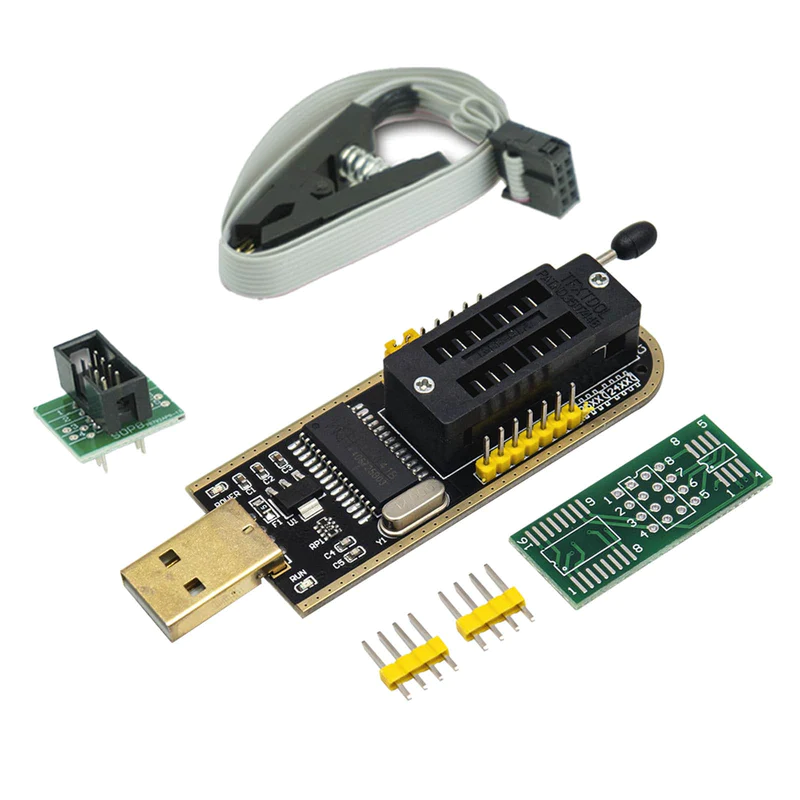
\includegraphics[scale=0.35]{programmer.png}
        \caption{Programador flash CH341A genérico.}
        \label{fig:programador}
    \end{figure}
    \item \textbf{Cifrado}: Además de no proporcionar un portal de descargas de firmware, los fabricantes también suelen cifrar sus paquetes de actualización para dificultar las 
    tareas de análisis e ingeniería inversa. Dicho firmware es posteriormente descifrado por la rutina de actualización del dispositivo. Cuando se da este caso desgraciadamente 
    solo quedan dos opciones, o extraer el firmware del mismo dispositivo como se ha comentado en el punto anterior o intentar obtener la versión del firmware previa a que el 
    fabricante implementara el cifrado en las actualizaciones y aplicar ingeniería inversa sobre la rutina de descifrado del firmware para llevar a cabo nuestra propia implementación. 
    \item \textbf{Formato}: Es bastante común para los fabricantes distribuir sus paquetes de firmware en formatos propietarios difíciles de tratar sin software especializado. 
    Binwalk\cite{binwalk} es una herramienta que puede ayudar con el análisis y desenpaquetado de imágenes firmware en binarios de los cuales se desconoce su estructura. El uso de esta herramienta
    será tratado a continuación. También es posible que se den casos en los que binwalk no sea capaz de identificar o extraer correctamente el contenido de la imagen firmware, 
    teniendo que recurrir al diseño de herramientas específicas para el firmware con el que se está trabajando, identificando los offsets a partir de dónde empiezan los distintos 
    componentes de este y extrayéndolos manualmente con herramientas como dd de las coreutils de GNU.
\end{itemize}

Para el Netgear R7000, es posible obtener el firmware a través de su \href{https://www.netgear.es/support/product/r7000.aspx#download}{portal oficial de soporte}. Una vez 
descargado el paquete de firmware versión 1.0.11.128, procedemos a su análisis con la herramienta Binwalk. El primer paso es comprobar si el binario se encuentra cifrado mediante 
la comprobación de su entropía. La entropía del binario es un valor que representa el nivel de aleatoriedad entre los bytes del fichero y un valor alto constante
en todo el binario es un fuerte indicativo de que o su contenido ha sido comprimido o que este ha sido cifrado. Para consultar la entropía representada en una gráfica usamos Binwalk con la siguiente orden. 
\begin{lstlisting}[language=bash]
  $ binwalk -E R7000-V1.0.11.128_10.2.112.chk
\end{lstlisting}

Como podemos apreciar en la figura \ref{fig:binwalkEnt}, Binwalk reporta una entropía considerablemente alta para el firmware. Para comprobar si estamos
ante un firmware cifrado intentamos identificar el contenido de este usando la flag ''-e'' en lugar de ''-E''. Al hacerlo, Binwalk es capaz de detectar 
la presencia de tres elementos dentro del firmware (figura \ref{fig:binwalkExt}), una primera entrada de nombre ''TRX firmware header'' que contiene metadatos
del firmware en formato TRX como un magic number, la versión de TRX en uso, longitud del header o un checksum CRC32 para comprobar la integridad del paquete. Sería posible
identificar qué información corresponde a cada campo consultando la documentación sobre el formato TRX\cite{firmwareFormat}, pero Binwalk ya hace este trabajo 
por nosotros. Además, Binwalk nos indica que estamos ante un firmware basado en Linux. A continuación identifica una sección de datos comprimidos usando LZMA, un algoritmo
de compresión sin pérdidas usado en este caso para comprimir la imagen del Kernel de Linux. Por último, tenemos el sistema de archivos del dispositivo en formato
SquashFS, un sistema de archivos de solo lectura utilizado en dispositivos de recursos limitados por sus capacidades de compresión. Tras la extracción, tenemos acceso 
al contenido del sistema de archivos (figura \ref{fig:R7000squashfs}), el cual sigue la jerarquía de directorios aplicada en sistemas Linux. Además, la imagen 
del Kernel también es extraída y haciendo uso de la herramienta ''strings'' de las Coreutils de GNU podemos comprobar que la versión del kernel en uso es la 
2.6.36.4\ref{fig:R7000kernel}, modificada con soporte adicional para SoCs de Broadcom basados en ARM.

\begin{figure}[H]
    \centering
    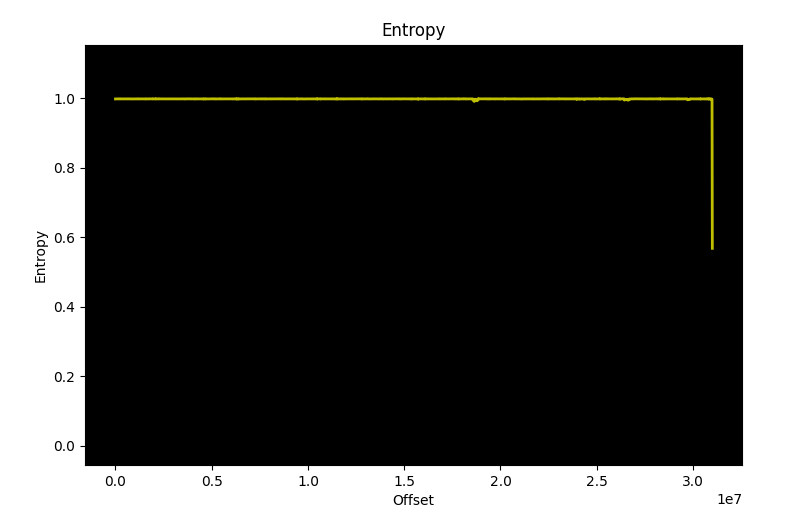
\includegraphics[scale=0.35]{r7000entropy.png}
    \caption{Gráfica de la entropía de la imagen firmware del Netgear R7000 generada por Binwalk.}
    \label{fig:binwalkEnt}
\end{figure}

\begin{figure}[H]
    \centering
    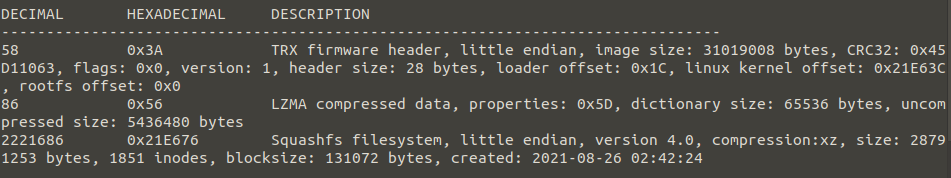
\includegraphics[scale=0.36]{r7000extraction.png}
    \caption{Extracción firmware Netgear R7000 usando Binwalk.}
    \label{fig:binwalkExt}
\end{figure}

\begin{figure}[H]
    \centering
    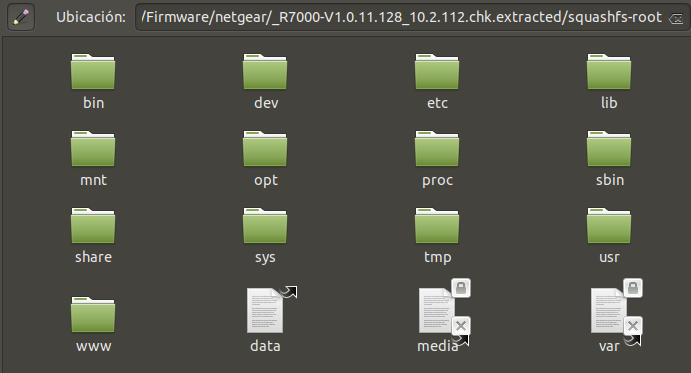
\includegraphics[scale=0.46]{r7000Squashfs.png}
    \caption{Sistema de archivos del Netgear R7000.}
    \label{fig:R7000squashfs}
\end{figure}

\begin{figure}[H]
    \centering
    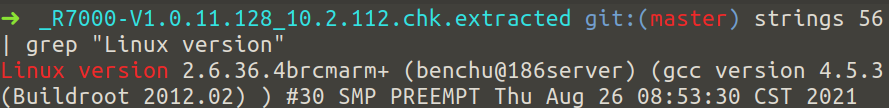
\includegraphics[scale=0.35]{r7000kernel.png}
    \caption{Versión del kernel utilizada por el R7000.}
    \label{fig:R7000kernel}
\end{figure}

Una vez extraído el firmware, podemos proceder a elegir un binario que nos resulte de interés para aplicarle fuzzing. Esto será
comentado en la siguiente sección.

\subsection{Introducción al experimento}
El experimento que va a ser realizado está basado en los descubrimientos realizados por el equipo de la firma de ciberseguridad GRIMM, publicados el
22 de Abril del 2022\cite{r7000GRIMM}. En su publicación, hacen una introducción a una vulnerabilidad detectada en el demonio UPNP presente en 
el firmware del Netgear R7000 en su versión 1.0.11.128 y anteriores. La vulnerabilidad se da concretamente en la funcionalidad de actualización de 
firmware proporcionada por el demonio UPNP y consiste en un buffer-overflow que puede llevar a ejecución remota de código (RCE) por parte de un usuario 
identificado en el sistema al proporcionar un paquete de actualización de firmware malicioso. Esto es posible debido a que la rutina de actualización 
al comprobar los headers confía en los tamaños especificados en la cabecera TRX\cite{firmwareFormat} incluida en el paquete de firmware proporcionado 
por el usuario para realizar operaciones de memoria. A continuación, aplican emulación full-system en QEMU con el objetivo de recrear la vulnerabilidad 
y diseñar una prueba de concepto de un firmware malicioso.\bigskip

El equipo de GRIMM identificó la vulnerabilidad mediante análisis estático de código haciendo uso de herramientas de decompilación como Ghidra\cite{Ghidra}.
Aunque se trata de una técnica efectiva, requiere de un experto cualificado que revise manualmente el código línea a línea y de un veredicto potencialmente 
incompleto. Como es lógico, no se trata de un procedimiento que pueda ser fácilmente escalable. Además, hacen uso de emulación full-system cuando solo desean
poner a prueba una pequeña parte de la funcionalidad del demonio. Es por ello que proponemos mejoras para ambos de los aspectos mencionados mediante la aplicación 
de técnicas alternativas. En primer lugar, respecto al procedimiento de identificación de la vulnerabilidad podemos hacer uso de fuzzing, realizando de forma 
automática mutaciones a la imagen del firmware que se proporciona a la rutina de actualización. Al aplicar fuzzing, posibilitamos la detección de vulnerabilidades 
similares a gran escala y ayudamos al revisor de código a evitar tener que analizar código superfluo pudiendo centrarse en analizar los crashes detectados por
el fuzzer, sabiendo ya que se trata de código problemático. En segundo lugar, podemos obtener una mejora de rendimiento sustituyendo la emulación full-system 
por el uso de técnicas basadas en Unicorn\cite{unicorn} que nos permitan instrumentar exactamente la rutina de actualización de firmware incluida en el 
demonio UPNP.\bigskip

En resumen, el objetivo del experimento es intentar identificar la misma vulnerabilidad pero haciéndolo a través de fuzzing, a la misma vez que comparamos el enfoque de 
emulación aplicado por el equipo de GRIMM con otras técnicas de emulación alternativas.

\subsection{Realización del experimento}
\subsubsection{Análisis del binario}
Comenzaremos por identificar el binario que implementa la funcionalidad del UPNP en el firmware y cargarlo en Ghidra\cite{Ghidra} para obtener una visión
decompilada o reconstruida del código original que nos permita encontrar la rutina de código que gestiona las actualizaciones del firmware. Para ello, 
accedemos al sistema de archivos que fue extraído del firmware previamente y abrimos con Ghidra el binario ubicado en ''usr/sbin/upnpd''. Una vez 
hecho esto, podemos guiar nuestra búsqueda por las cadenas de texto de mensajes de log presentes en el binario. Utilizando la funcionalidad de búsqueda 
de strings en Ghidra podemos buscar strings relacionadas con términos como ''firmware'', ''header'', ''update'' o similares. Dado que la vulnerabilidad 
se da a la hora de comprobar los headers del firmware, buscamos por ''header'' y rápidamente identificamos el string ''Header checksum error!!!'' 
siendo referenciado por dos funciones distintas (figura \ref{fig:R7000string}).

\begin{figure}[H]
    \centering
    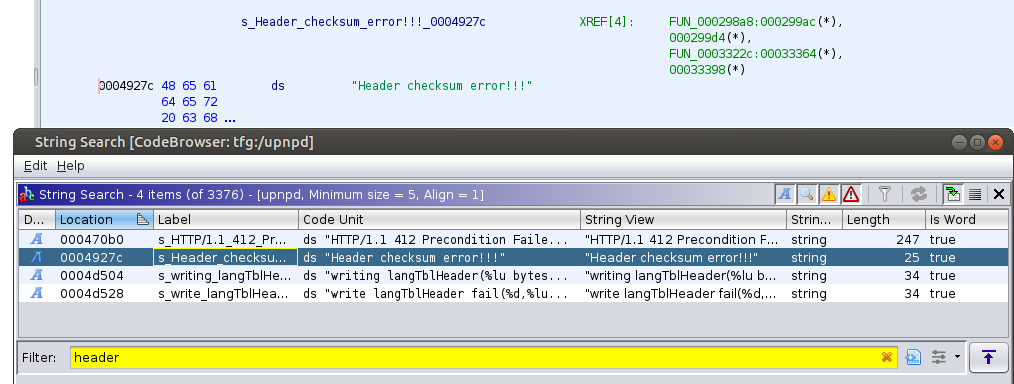
\includegraphics[scale=0.35]{r7000string.png}
    \caption{Resultados de la búsqueda de strings en Ghidra.}
    \label{fig:R7000string}
\end{figure}

Ambas funciones implementan aparentemente la misma lógica de parsing de la cabecera del firmware con la única diferencia de que ''FUN\_0003322c''
(figura \ref{fig:R7000decompilado}) contiene hardcodeado el modelo del dispositivo para compararlo con un valor incluido en el firmware. 
Ya que esta función parece destinada a nuestro modelo específico, será la función que usemos como objeto de pruebas más adelante y la apodaremos 
''check\_upd\_header''. Realizando un breve 
análisis del código decompilado, podemos observar que en la línea 17 se comprueba una cadena mágica para verificar que se trata de un firmware, 
en las líneas 29 y 30 se realizan operaciones con memoria que analizaremos más adelante y de la línea 34 a la 44 se llevan a cabo comprobaciones de que 
el firmware corresponda con el modelo de dispositivo en el que va a ser instalado.

\begin{figure}[H]
    \centering
    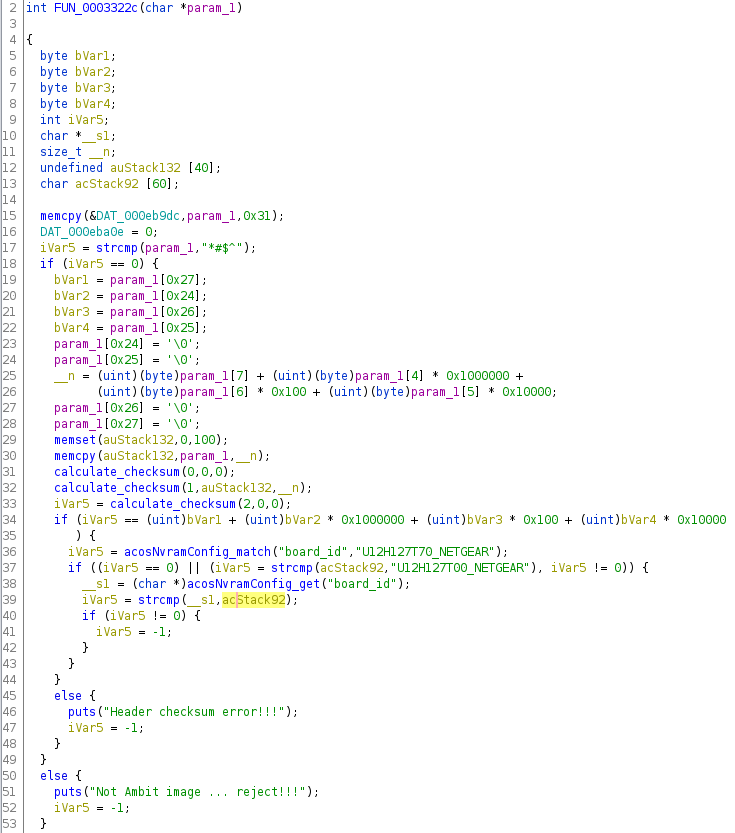
\includegraphics[scale=0.45]{r7000decompilado.png}
    \caption{Función del UPNP decompilada por Ghidra.}
    \label{fig:R7000decompilado}
\end{figure}

\subsubsection{Emulación del binario}
Es imprescindible conseguir emular el binario como paso previo a aplicar fuzzing sin disponer del dispositivo original. Para ello, como se ha comentado 
anteriormente pondremos a prueba tanto la metodología de emulación QEMU full-system propuesta por GRIMM en su artículo como una emulación mediante 
Qiling\cite{qiling} que en lugar de emular el demonio en su totalidad, instrumente el binario para ejecutar exclusivamente la función que hemos identificado 
en la sección anterior. Además, pondremos a prueba la efectividad de FirmAE\cite{Kim2020} para comprobar si pudiera proporcionar una mejor experiencia de 
emulación full-system en comparación con QEMU básico.

\paragraph{Qiling}
Para emular la función deseada con Qiling, aplicaremos la misma técnica que ha sido desarrollada para instrumentar el código en la prueba de concepto anterior, es decir, se harán uso 
de dos hooks para alterar el flujo de ejecución del código. El primer hook se ejecutará al llegar al punto de entrada del ejecutable y reemplazará el primer 
parámetro de la función (registro R0 según la convención de llamada a funciones en ARM32) con la dirección en hexadecimal de check\_upd\_header() para convertir 
la función en el main del programa. El segundo hook también sigue el mismo funcionamiento, dado que check\_upd\_header() solo recibe como parámetro un array 
de bytes representando el header del firmware, solo será necesario alocar manualmente los bytes que el script de Qiling haya leído de un archivo que se le 
pase por línea de comandos. En la figura \ref{fig:R7000flowchart} podemos observar el flujo de ejecución aplicando instrumentación 
dinámica con el script de Qiling.

\begin{figure}[H]
    \centering
    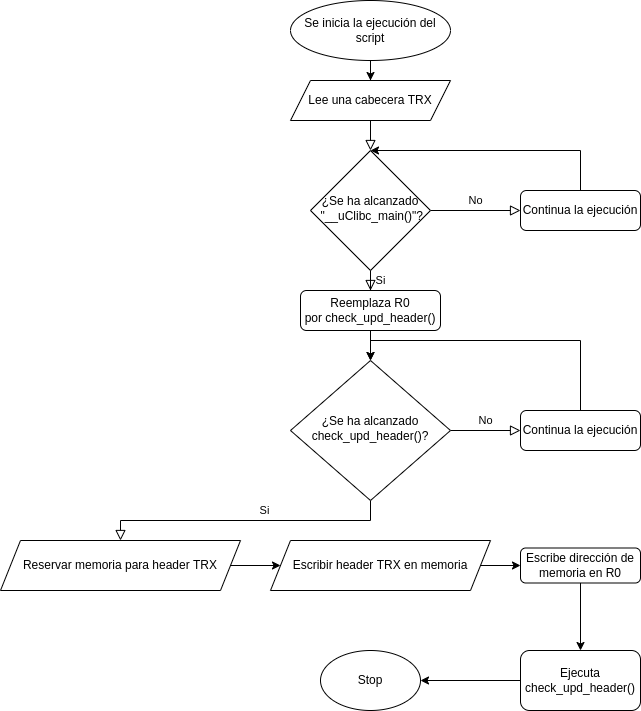
\includegraphics[scale=0.45]{r7000flowchart.png}
    \caption{Diagrama de flujo representando la instrumentación realizada sobre UPNP.}
    \label{fig:R7000flowchart}
\end{figure}

Para crear el script, empezamos consultando en Ghidra la dirección de la función ''\_\_uClibc\_main()'' y las direcciones de 
inicio y fin de la función target check\_upd\_header() para crear variables reconocibles en el script. Para el caso de este 
binario, las direcciones son las siguientes:

\begin{lstlisting}[language=python, caption=Declaración de constantes: Direcciones de interés en funciones., captionpos=b,
     frame=single, breaklines]
    TARGET_FUNC_ADDR    = 0x3322c   # Address of the function we are interested in
    TARGET_END_ADDR     = 0x33360   # End fuzzing when reaching this address
    LIBC_START_ADDR     = 0x0c460   # Address where __uClibc_main is being called
\end{lstlisting}

Gracias a la intuitiva API de Qiling, establecer los hooks es tan fácil como asociar la dirección de una instrucción del binario
con una función del script. También cabe mencionar que definiremos como ''rootfs'' la ruta al sistema de archivos extraído del
firmware previamente para que el enlazado dinámico de librerías se produzca correctamente. Definimos de la siguiente manera los
hooks y sus funciones asociadas.

\begin{lstlisting}[language=python, caption=Definición de hooks del script de emulación para Qiling., captionpos=b,
    frame=single, breaklines]
    def libc_start_main_redirect(ql: Qiling, func_addr = TARGET_FUNC_ADDR):
    ql.reg.write("r0", func_addr)
    
    def indirect_write_reg_bytes(ql: Qiling, register_id, bytes):
        address = ql.mem.map_anywhere(len(bytes))
        ql.mem.write(address, bytes)
        ql.reg.write(register_id, address) # == (ql.reg.r0 = address) 

    def target_hook(ql: Qiling):    
        print("\n--------------\n")
        print("HOOK, PC: 0x%x" % ql.reg.arch_pc)
        print("Using", PAYLOAD, "as payload\n")
        indirect_write_reg_bytes(ql, "r0", PAYLOAD)
        print("\n--------------\n")
        
    def sandbox(path, rootfs, debug):    
        ql = Qiling(path, rootfs)
        ql.hook_address(libc_start_main_redirect, LIBC_START_ADDR)
        ql.hook_address(target_hook, TARGET_FUNC_ADDR)     
        ql.debugger = debug
        ql.run(end=TARGET_END_ADDR)

    ...
\end{lstlisting}

Tras crear el script, necesitaremos un sample de cabeceras de firmware para pasarle a este como parámetro y comprobar así
su funcionamiento. Para ello, simularemos un caso de actualización de firmware real, es decir, descargaremos el paquete de 
firmware correspondiente a la siguiente versión (1.0.11.128 -> 1.0.11.134) y extraeremos los mil primeros bytes de este ya que 
solo estamos interesados en las cabeceras y el inicio del fichero. DD permite hacer esto con la siguiente orden:

\begin{lstlisting}[language=bash, breaklines]
    $ dd if=R7000-V1.0.11.134_10.2.119.chk of=header134.chk count=1 bs=1K
\end{lstlisting}

Mirando el volcado en hexadecimal del fichero resultante (figura \ref{fig:R7000header}), saltan rápidamente a la vista dos de
los campos descritos anteriormente al tratar la estructura de una cabecera TRX y las comprobaciones previas que realiza 
check\_upd\_header(), el magic number al inicio del fichero con el valor ''*\#\$\textasciicircum'' y el modelo de dispositivo
para el que va destinada la actualización ''U12H270T00\_NETGEARHDR0''.

\begin{figure}[H]
    \centering
    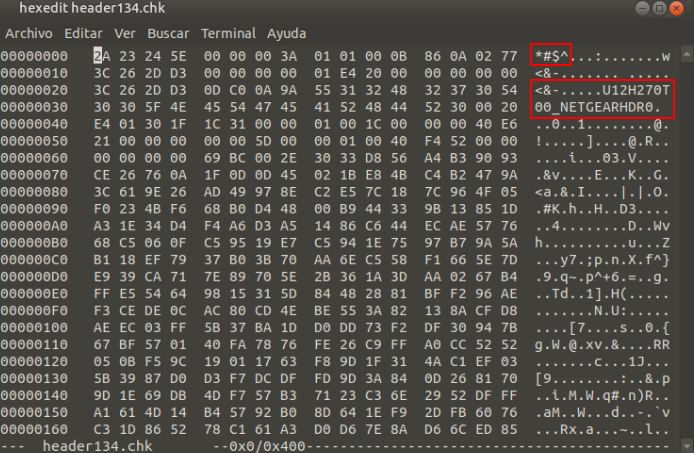
\includegraphics[scale=0.5]{r7000header.png}
    \caption{Representación hexadecimal del contenido del firmware.}
    \label{fig:R7000header}
\end{figure}

A continuación, podemos ejecutar el script y comprobar su funcionamiento. Al ejecutarlo pasando como parámetro 
''header134.chk'' (figura \ref{fig:R7000qiling}), observamos que los hooks se aplican correctamente y aunque la ejecución 
parece finalizar correctamente se muestran errores ENOENT debido a la ausencia de una NVRAM en ''/dev/nvram''. Esto se produce cuando la función emulada
intenta consultar en la NVRAM la variable ''board\_id'' para compararla con el string del modelo en el firmware comentado
anteriormente. Dado que no estamos emulando la NVRAM ni haciendo uso de librerías alternativas como nvram-faker\cite{nvram}
para interceptar las operaciones con este dispositivo, se producen errores al intentar consultar variables en este pero ya
que solo se utiliza para realizar la comparación de ambas cadenas, podemos ignorar los errores por el momento.

\begin{figure}[H]
    \centering
    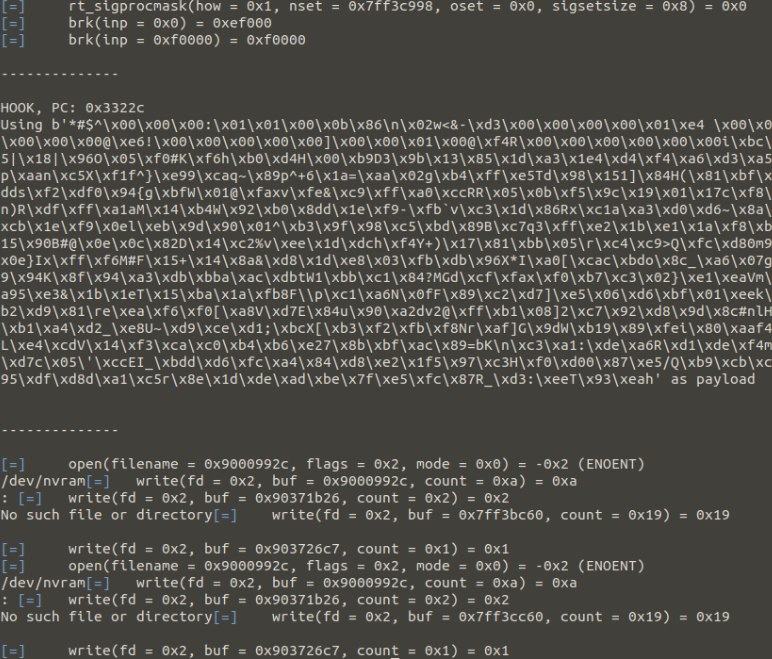
\includegraphics[scale=0.4]{r7000qiling.png}
    \caption{Resultado de la emulación de check\_upd\_header() con Qiling.}
    \label{fig:R7000qiling}
\end{figure}

Si probamos a modificar la cadena mágica del firmware y a pasárselo al script, comprobamos que efectivamente se avisa de que 
el fichero no se trata de una actualización de firmware válida (figura \ref{fig:R7000magic}), cancelando así el proceso de actualización si estuviéramos 
emulando el binario al completo.

\begin{figure}[H]
    \centering
    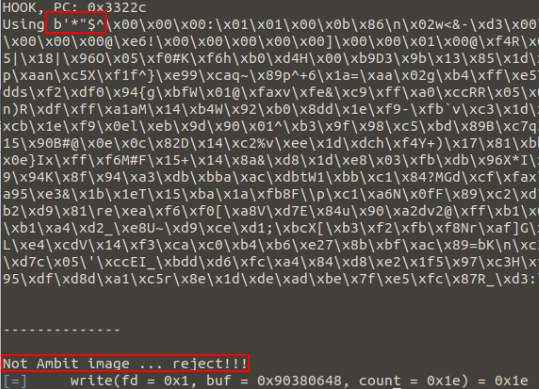
\includegraphics[scale=0.65]{r7000magic.png}
    \caption{Fallo al comprobar la cadena mágica en Qiling.}
    \label{fig:R7000magic}
\end{figure}

\paragraph{QEMU}
Para emular el firmware aplicando emulación full-system en QEMU, es más viable obtener una máquina virtual Linux para sistemas ARM 
y ejecutar en esta los binarios de interés antes que intentar emular el firmware del dispositivo al completo, debido a la 
necesidad de tener que manualmente solucionar los problemas de compatibilidad por aspectos como diferencias en la configuración 
de interfaces red o la ausencia de dispositivos necesarios durante el arranque del sistema como hemos comprobado anteriormente 
con el NVRAM. Por ello, partimos de una VM de Debian ARM (debian-10-openstack-arm64.qcow2) obtenida de su  
\href{https://cdimage.debian.org/cdimage/cloud/OpenStack/}{web oficial} en la que introduciremos el sistema de archivos extraído del firmware 
del R7000 para ejecutar el binario del servicio UPNP teniendo todas las librerías necesarias para ello. Utilizamos la siguiente 
orden para arrancar la máquina virtual descargada con 2GB de RAM, todos los núcleos disponibles de la CPU, almacenamiento, un 
adaptador de red y los puertos 22 y 5000 redirigidos a la máquina host. El puerto 22 será de utilidad para acceder 
mediante SSH a la máquina virtual mientras que el 5000 lo necesitamos para poder realizar peticiones por el protocolo SOAP, que 
es el protocolo utilizado por el demonio UPNP para interactuar con este desde el exterior.

\begin{lstlisting}[language=bash, breaklines]
    $ qemu-system-aarch64 -m 2G -M virt -cpu max -bios /usr/share/qemu-efi-aarch64/QEMU_EFI.fd -drive if=none,file=debian-10-openstack-arm64.qcow2,id=hd0 -device virtio-blk-device,drive=hd0 -device e1000,netdev=net0 -netdev user,id=net0,hostfwd=tcp:127.0.0.1:1234-:22,hostfwd=tcp::5000-:5000 -nographic
\end{lstlisting}

\begin{figure}[H]
    \centering
    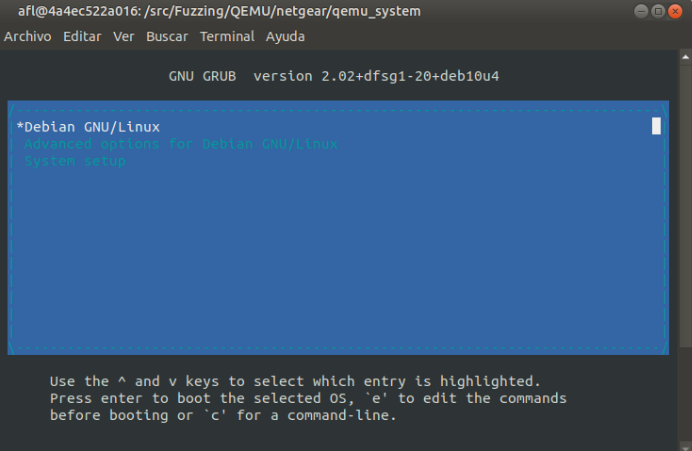
\includegraphics[scale=0.55]{r7000QemuBoot.png}
    \caption{Grub menu from the ARM QEMU VM.}
    \label{fig:R7000QemuBoot}
\end{figure}

Al finalizar el arranque de la máquina virtual, podemos utilizar \textit{chroot} para cambiar el directorio raíz actual al directorio 
del sistema de archivos extraído del router previamente (figura \ref{fig:R7000shell}). Desafortunadamente, al poner en marcha el 
servicio del UPNP comprobamos que no es capaz de funcionar correctamente en el entorno virtual actual. Como documenta GRIMM\cite{r7000GRIMM}
en sus descubrimientos, esto se debe a una mala configuración de las interfaces red y a la falta de una NVRAM desde la que leer los 
parámetros de configuración del servicio. Este tipo de problemas son de esperar al aplicar técnicas de emulación full-system y han 
de ser solventados para conseguir que el demonio se ejecute correctamente.

\begin{figure}[H]
    \centering
    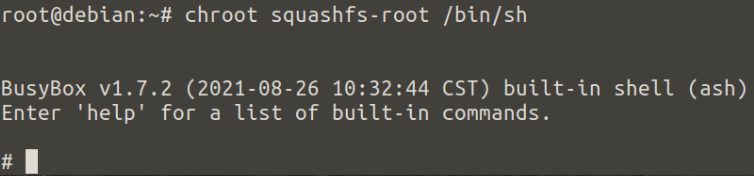
\includegraphics[scale=0.55]{r7000shell.png}
    \caption{Busybox shell desde el sistema de archivos del R7000.}
    \label{fig:R7000shell}
\end{figure}

Para solucionar estos problemas haremos uso de las soluciones proporcionadas por el equipo de GRIMM\cite{r7000GRIMM}. En primer
lugar, modificaremos el flujo de ejecución del binario con GDB para evitar llamar a \textit{exit()} al fallar el bloque de código 
que realizar la comprobación de las interfaces de red. Como podemos ver en la versión decompilada del código que realiza dicha 
comprobación mostrada en la figura \ref{fig:R7000iffix}, será necesario establecer un breakpoint al llegar a ''FUN\_0000e4c8''
para que cuando esto suceda, cambiar el contador de programa a la dirección del return de la función con el objetivo de saltarnos 
la comprobación. Para solucionar la falta de una NVRAM, reemplazaremos la librería dinámica ''libnvram.so'' del sistema de archivos 
por una versión modificada de nvram-faker\cite{nvram} que GRIMM proporciona con las variables extraídas de un dispositivo original.
Esto resulta un claro punto negativo para la aplicación de emulación full-system, ya que para conseguir que nuestro binario de 
interés se ejecute correctamente, hubiéramos necesitado disponer del dispositivo original e identificar todas las variables 
consultadas en la NVRAM y sus valores esperados a través de ingeniería inversa y análisis estático de código no resulta viable. 

\begin{figure}[H]
    \centering
    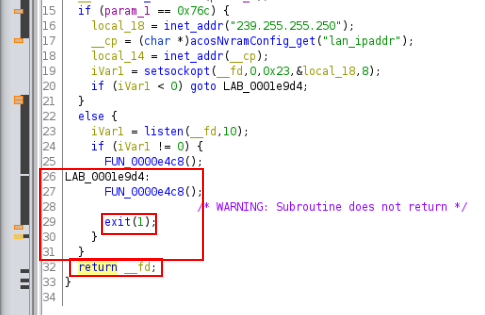
\includegraphics[scale=0.65]{r7000iffix.png}
    \caption{Rutina de comprobación de interfaces de red R7000.}
    \label{fig:R7000iffix}
\end{figure}

Tras solucionar los problemas encontrados, hacemos uso de la siguiente orden para automatizar el proceso de hacer \textit{chroot}
al sistema de archivos, ejecutar UPNP en segundo plano, attachear GDB a este proceso y llevar a cabo el cambio de flujo descrito.
Esta vez, ya es posible realizar peticiones por el puerto 5000 al servicio a través de CURL (figura \ref{fig:R7000QemuWorking}). Por ahora nos sirve 
con saber que el servicio es capaz de responder peticiones pero más adelante, crearemos un script para llevar a cabo las peticiones 
SOAP necesarias a través de HTTP para iniciar la funcionalidad de actualización de firmware.

\begin{lstlisting}[language=bash, breaklines]
    $ chroot squashfs-root /bin/sh -c "/usr/sbin/upnpd&" && gdb -x ./gdb_script -q -p `pgrep upnpd`
\end{lstlisting}

\begin{figure}[H]
    \centering
    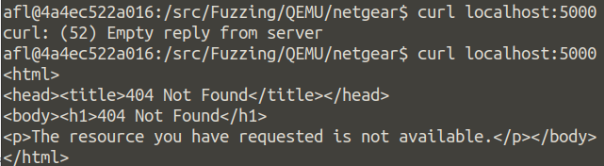
\includegraphics[scale=0.65]{r7000QemuWorking.png}
    \caption{UPNP respondiendo una petición GET básica.}
    \label{fig:R7000QemuWorking}
\end{figure}

\paragraph{FirmAE}
Como se comentó en el apartado ''\nameref{estado_del_arte}'', FirmAE fue desarrollado con el objetivo de poder solucionar mediante heurísticas 
pequeños problemas de configuración como los que hemos experimentado al intentar emular el binario con QEMU básico. Por ello, 
procederemos a poner esta herramienta en práctica para comprobar si supone alguna mejoría con respecto a la metodología seguida
por GRIMM\cite{r7000GRIMM}.\bigskip

Iniciar la emulación del firmware con FirmAE es tan simple como indicarle la ruta a la imagen firmware del dispositivo. A continuación, 
FirmAE analiza dinámicamente el firmware durante aproximadamente diez minutos para intentar detectar problemas de configuración y 
ajustar el entorno de emulación con el objetivo de satisfacer sus necesidades (figura \ref{fig:R7000FirmAE}). 

\begin{figure}[H]
    \centering
    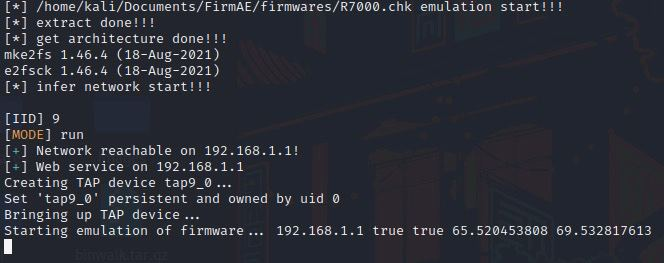
\includegraphics[scale=0.54]{r7000FirmAE.png}
    \caption{Instancia de FirmAE emulando el firmware de un R7000.}
    \label{fig:R7000FirmAE}
\end{figure}

Al intentar acceder a la dirección IP local que ha habilitado FirmAE para el portal web del dispositivo, nos encontramos con el proceso de 
setup original de Netgear (figura \ref{fig:R7000Setup}) el cual no podemos completar porque el resto del proceso de configuración se lleva a cabo
en la dirección ''www.routerlogin.net'' y se asume que se está utilizando el servidor DNS del router emulado, por lo que no se nos redirige 
correctamente a la configuración al visitar dicha dirección. Esto puede solucionarse editando el fichero ''/etc/hosts'' en Linux para que 
el hostname ''routerlogin.net'' resuelva a la dirección IP asignada por FirmAE. Tras este cambio somos capaces de finalizar el setup inicial 
y de acceder al panel de control del router (figura \ref{fig:R7000panel}). 

\begin{figure}[H]
    \centering
    
\includegraphics[scale=0.5]{r7000Setup.png}
    \caption{Setup de configuración del R7000.}
    \label{fig:R7000Setup}
\end{figure}

\begin{figure}[H]
    \centering
    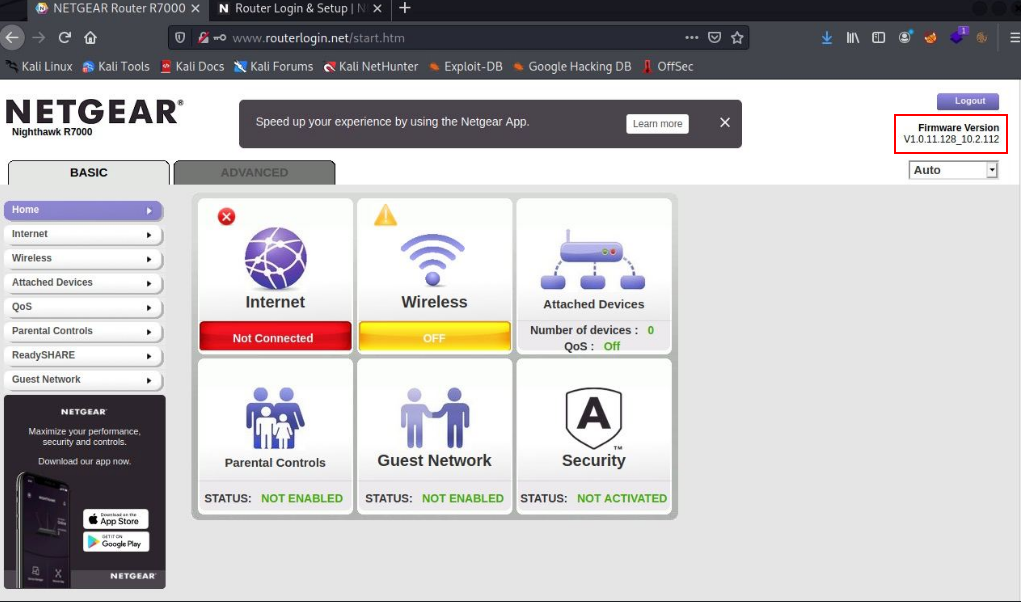
\includegraphics[scale=0.45]{r7000panel.png}
    \caption{Panel de control del R7000.}
    \label{fig:R7000panel}
\end{figure}

Por desgracia, aunque el portal web principal parece estar siendo correctamente emulado, solo obtenemos ''empty response'' al realizar peticiones
por el puerto 5000 al demonio UPNP. Ejecutando manualmente el binario desde la shell proporcionada por FirmAE, observamos que la ejecución 
entra en un bucle infinito intentando llevar a cabo operaciones en exclusión mutua relacionadas con el uso de variables de la NVRAM 
(figura \ref{fig:R7000FirmAEupnp}). Dado que el problema sigue presente incluso al usar nvram-faker\cite{nvram}, la emulación del firmware
a través de FirmAE queda descartada.

\begin{figure}[H]
    \centering
    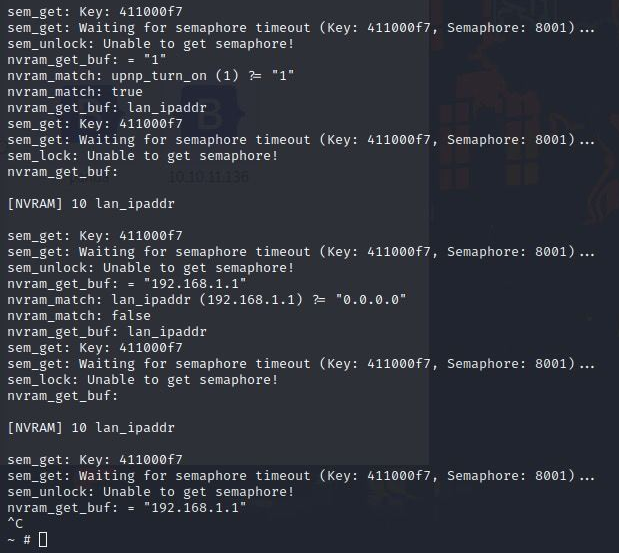
\includegraphics[scale=0.5]{r7000FirmAEupnp.png}
    \caption{Bucle infinito al ejecutar UPNP con FirmAE.}
    \label{fig:R7000FirmAEupnp}
\end{figure}

\subsubsection{Aplicación de fuzzing}
Tras conseguir emular el servicio UPNP del firmware aplicando tanto emulación full-system en QEMU como emulación basada en Unicorn\cite{unicorn}
con Qiling\cite{qiling}, procederemos a aplicar fuzzing sobre dicho servicio con el objetivo de explorar otras técnicas a partir de las cuales 
se podría haber llegado a esta vulnerabilidad además de compararlas entre sí.

\paragraph{Vulnerabilidad a identificar} Como se ha comentado en la introducción al experimento, buscamos alcanzar a través de fuzzing una 
vulnerabilidad previamente conocida y gracias a que partimos sabiendo qué se trata buscar, procederemos a analizar brevemente dicha vulnerabilidad
sobre el código decompilado (figura \ref{fig:UpnpCheckHeader}) con el objetivo de facilitar al lector la comprensión del experimento, los problemas encontrados y los resultados de este. 
El funcionamiento de ''check\_upd\_header()'' puede dividirse en cinco pasos principales. En primer lugar, se comprueba que el firmware tenga 
la cadena mágica ''*\#\$\textasciicircum'' al inicio mediante una llamada a la función \textit{strcmp} sobre el array de bytes que representa al 
firmware. Esto es posible debido a que las cadenas de caracteres en C vienen delimitadas por un byte nulo al final y recordemos que los campos de 
las cabeceras TRX\cite{firmwareFormat} vienen también delimitadas por bytes nulos. En el segundo paso observamos como se utiliza la siguiente 
sección de la cabecera para obtener el tamaño de esta. El principal problema de este paso y el factor que causa la vulnerabilidad que estamos tratando
es la ausencia de validación de los datos que están siendo recibidos del exterior los cuales nunca deberían de ser confiados, aún menos cuando 
ese input va a ser utilizado como parámetro en operaciones con memoria a continuación en el tercer paso. Dado que el usuario desde el exterior
puede fijar cuantos bytes van a ser copiados sobre el buffer de destino, este podría provocar un desbordamiento de la pila, pudiendo también modificar la 
dirección de retorno de la función además de diversos registros usados para almacenar variables locales en ARM32 (R4-R11). Por último, en los pasos 
cuatro y cinco se llevan a cabo comprobaciones adicionales sobre el checksum y el modelo del dispositivo para evitar que el usuario aplique un paquete
de firmware incorrecto o corrompido.

Para que un fuzzer sea capaz de identificar el crash producido por el desbordamiento de la pila, este tendrá que generar un input mutado que respete la 
cadena mágica inicial además de incluir en el campo del tamaño de la cabecera un valor superior al admitido por el buffer de destino ubicado en la pila.

\begin{figure}[H]
    \centering
    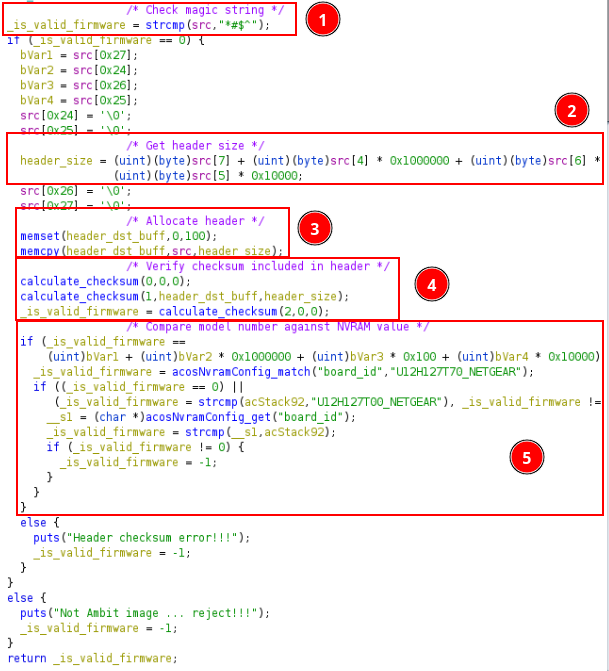
\includegraphics[scale=0.55]{UpnpCheckHeader.png}
    \caption{Decompilado de la función ''check\_upd\_header()'' comentado.}
    \label{fig:UpnpCheckHeader}
\end{figure}

\paragraph{Fuzzing con Qiling}
Para realizar fuzzing usando Qiling, partimos del script que ha sido desarrollado previamente para la emulación e instrumentación del binario al
cual se le realizarán algunas modificaciones para integrar la lectura de inputs con un fuzzer de caja gris como es AFL++\cite{afl++}. Además, también se 
creará una versión del script que utilice a Radamsa\cite{radamsa} como generador de inputs para poder comprobar si un fuzzer de caja negra
pudiera dar mejores resultados que uno de caja gris en determinadas situaciones.\bigskip

Empezando por integrar el script de Qiling con AFL++, haremos uso de los bindings para Python que proporciona AFL++ como parte de su integración
con Unicorn. El flujo de ejecución será el mismo, con la diferencia de que el almacenamiento de los bytes del header en memoria se hará ahora 
dentro de un callback que será llamado por AFL++ cada vez que este desee realizar una nueva iteración durante el fuzzing. De esta forma hacemos
uso de dos hooks, un primer hook que lleva a cabo el cambio del punto de entrada del binario de la misma forma que en el script de emulación y un 
segundo que llama a una función encargada de reportar a AFL++ que se ha llegado al punto de inicio para el fuzzing. Por último, adelantamos la 
dirección en la que finaliza la ejecución del binario modificando ''TARGET\_END\_ADDR'' para evitar realizar las comparaciones del modelo del 
dispositivo, ya que de todas formas no estaban siendo emuladas correctamente al carecer de una NVRAM. Tener que emular un menor número de 
instrucciones por ejecución del script supone una mejora en el número de ejecuciones por segundo. El script resultante es el siguiente donde 
''place\_input\_callback()'' es la función llamada por AFL++ para almacenar los inputs mutados en memoria y ''start\_afl()'' la función a ejecutar 
al llegar ''check\_upd\_header()'' para comenzar una nueva iteración de fuzzing.

\begin{lstlisting}[language=python, caption=Script de fuzzing de UPNP para Qiling., captionpos=b,
    frame=single, breaklines, showstringspaces=false]
    import sys, os
    from qiling import Qiling
    from qiling.extensions.afl import ql_afl_fuzz
    
    TARGET_FUNC_ADDR    = 0x3322c   # Address of the function we are interested in
    TARGET_END_ADDR     = 0x3330c   # End fuzzing when reaching this address
    LIBC_START_ADDR     = 0x0c460   # Address where __libc_start_main is being called
        
    def libc_start_main_redirect(ql: Qiling, func_addr = TARGET_FUNC_ADDR):
        ql.arch.regs.write("r0", func_addr)
        
    def sandbox(path, rootfs, debug, param_file):
        ql = Qiling(path, rootfs)
        ql.hook_address(libc_start_main_redirect, LIBC_START_ADDR)
        
        def place_input_callback(_ql: Qiling, input: bytes, _):
            address = _ql.mem.map_anywhere(len(input))
            
            print("\n\n FILE LENGTH (bytes): ", len(input))
            
            _ql.mem.write(address, input)
            _ql.arch.regs.write("r0", address)
            
            res = _ql.mem.read(address, len(input));
            print("\n\n FUNCTION INPUT BYTES: \n\n", input)
            print("\n\n BYTES STORED IN MEMORY: \n\n", res)
            
        def start_afl(_ql: Qiling):
            ql_afl_fuzz(_ql, param_file, place_input_callback, exits=[ql.os.exit_point])
        
        ql.hook_address(start_afl, TARGET_FUNC_ADDR)
    
        try:
            ql.run()
            os._exit(0)
        except:
            os._exit(1)
        
        ...
\end{lstlisting}

Gracias a nuestro script, podemos iniciar una sesión de fuzzing en AFL++ (figura \ref{fig:R7000QilingFuzz}) con la siguiente orden, donde ''fuzz\_setup/in''
es un directorio que contiene un corpus formado por los primeros 1024 bytes de las dos imágenes del firmware en sus versiones 1.0.11.128 y 1.0.11.134,
mientras que ''fuzz\_setup/out'' será el directorio donde AFL++ almacene los resultados de la sesión de fuzzing (crashes o timeouts identificados, estadísticas de 
la sesión\dots). Además, con el objetivo de reducir el número de inputs que son descartados prematuramente en la comprobación de la cadena mágica, 
hacemos uso de la funcionalidad de diccionarios de AFL++ (flag -x) con un diccionario que contenga la cadena ''*\#\$\textasciicircum''.
\begin{lstlisting}[language=bash, breaklines]
    $ afl-fuzz -i fuzz_setup/in -o fuzz_setup/out -x dict/dictionary -U -- python3 ./src/dev/fuzz.py @@
\end{lstlisting}

Viendo que el fuzzing se realiza correctamente y que se descubren nuevos paths a explorar en el código, procedemos a dejar la 
sesión de fuzzing corriendo hasta que llegue el punto en el que AFL++ no detecte nuevos sucesos durante el fuzzing. AFL++ indica cuándo
esto sucede a través del color de la variable ''cycles done'', la cual cambia a color verde cuando no se ha alcanzado nuevo código 
ni se han visto diferencias en el comportamiento de este durante un tiempo. En este caso, el tiempo que se dedicó al proceso de fuzzing 
fue un total de 20 horas y 31 minutos corriendo en modo paralelo con 3 instancias del fuzzer simultáneas (\ref{fig:R7000parallel}).

\begin{figure}[H]
    \centering
    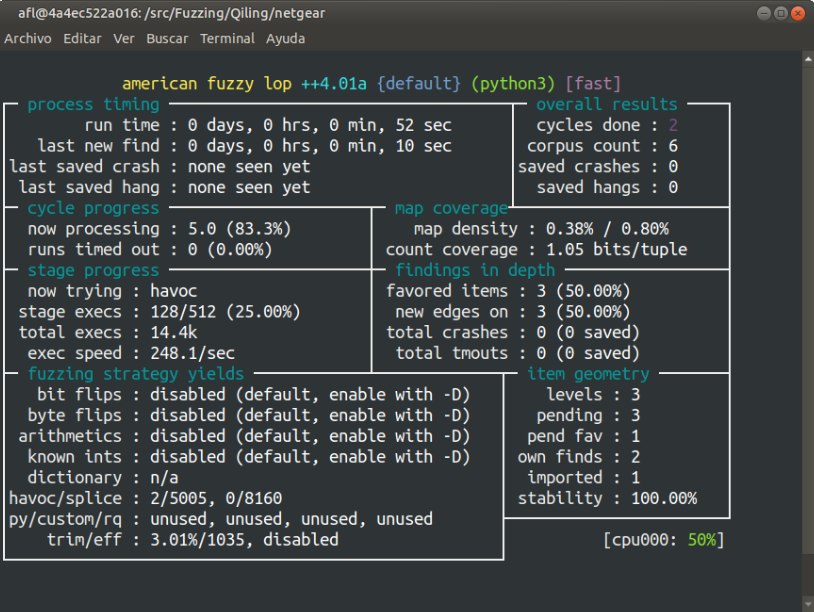
\includegraphics[scale=0.5]{r7000QilingFuzz.png}
    \caption{Sesión de fuzzing sobre UPNP usando Qiling.}
    \label{fig:R7000QilingFuzz}
\end{figure}

\begin{figure}[H]
    \centering
    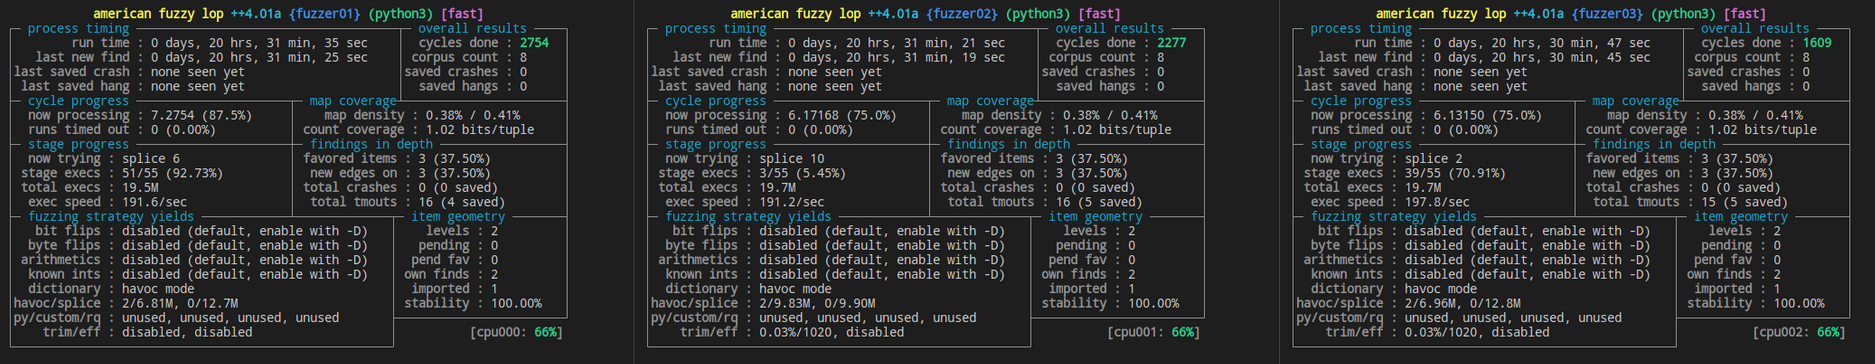
\includegraphics[scale=0.25]{AFLparallel.png}
    \caption{Sesión de fuzzing sobre UPNP con tres instancias en paralelo.}
    \label{fig:R7000parallel}
\end{figure}

\paragraph{Fuzzing con QEMU full-system}
Para este caso desarrollaremos un script en Python que nos permita llevar a cabo repetidas peticiones HTTP
al servicio UPNP mutando exclusivamente el firmware enviado. Para el aspecto de la generación de
inputs utilizaremos el fuzzer de caja negra Radamsa\cite{radamsa} debido a su excelente algoritmo 
de mutación además de estar diseñado para ser fácilmente integrable con scripts. Este experimento nos 
permitirá comprobar si la información adicional de feedback utilizada en el fuzzing de caja gris es 
de utilidad para este caso en comparación con el fuzzing de caja negra.\bigskip

El script a desarrollar deberá de en primer lugar, iniciar sesión en el servicio UPNP para obtener una cookie de sesión
previamente a mutar el firmware y enviarlo. Ya que UPNP trabaja en este caso mediante el protocolo SOAP a través de HTTP,
tendremos que realizar peticiones que sigan el formato correspondiente como podemos observar en la figura \ref{fig:SOAPlogin}
para la obtención de la cookie de sesión y en la figura \ref{fig:SOAPupdate} para iniciar la actualización de firmware.
Ambas peticiones serán tratadas más en profundidad a continuación con el desarrollo del script.

\begin{figure}[H]
    \centering
    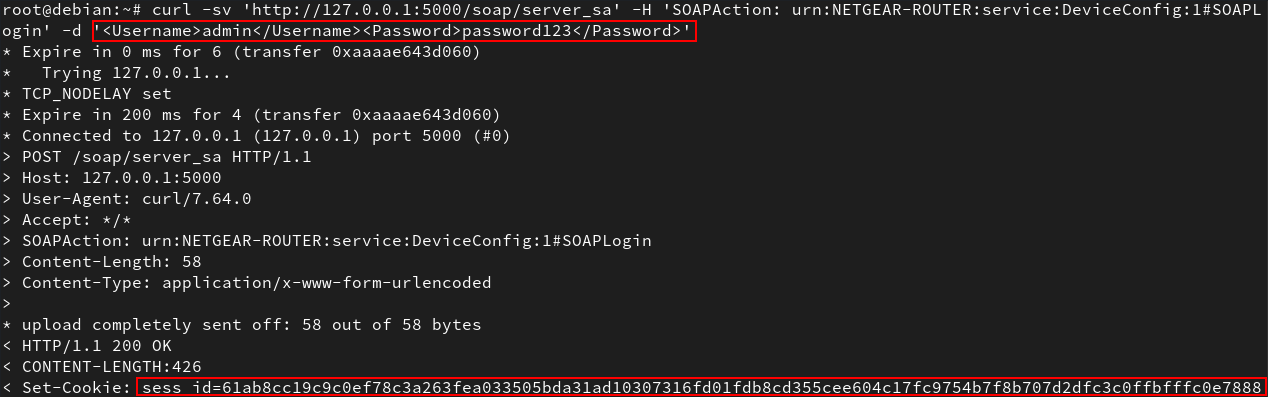
\includegraphics[scale=0.35]{SOAPlogin.png}
    \caption{Petición de login al servicio UPNP.}
    \label{fig:SOAPlogin}
\end{figure}

\begin{figure}[H]
    \centering
    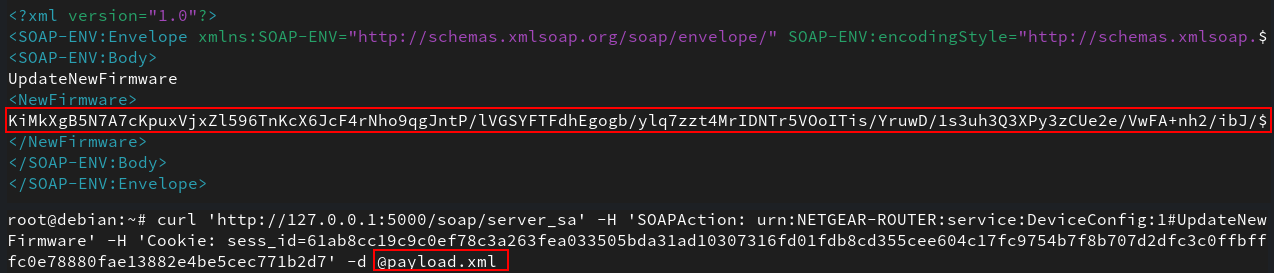
\includegraphics[scale=0.35]{SOAPupdate.png}
    \caption{Petición de actualización de firmware al servicio UPNP.}
    \label{fig:SOAPupdate}
\end{figure}

La función ''login()'' de nuestro script enviará una petición HTTP al endpoint 
''http://127.0.0.1:5000/soap/server\_sa'', indicando en la cabecera que la acción SOAP a realizar es ''SOAPLogin''
e incluyendo en los datos de la petición el usuario y contraseña por defecto del administrador. Una vez 
recibida la respuesta, extraemos el valor de la cookie ''sess\_id'' para realizar posteriormente peticiones
autenticadas.

\begin{lstlisting}[language=python, caption=Función para realizar login en el servicio UPNP., captionpos=b,
    frame=single, breaklines, showstringspaces=false]
    def login():
        url = 'http://127.0.0.1:5000/soap/server_sa'
        header = {'SOAPAction': 'urn:NETGEAR-ROUTER:service:DeviceConfig:1#SOAPLogin'}
        data = '<Username>admin</Username><Password>password123</Password>'
        
        response = requests.post(url, headers=header, data=data)
        cookie = response.cookies.get_dict()["sess_id"]
        return cookie
\end{lstlisting}

La función ''sendUpdate()'' iniciará el proceso de actualización de firmware mandando la petición correspondiente al 
UPNP. Para ello, se enviará otra petición al mismo endpoint ahora con la acción SOAP ''UpdateNewFirmware'' en el header,
incluyendo la cookie de sesión obtenida por la función ''login()'', además del firmware codificado en base64 como parámetro 
de la petición dentro de un XML. Dado el enfoque de caja negra que estamos aplicando en este caso, la forma en la que comprobamos 
si la petición realizada ha producido algún efecto adverso en el servicio es realizando un liveness-check con la función ''crashTest()''
cuando el servicio no ha respondido correctamente nuestra petición de actualización de firmware. De esta forma, si se produce algún error
en la conexión, se realizará una simple petición HTTP al servicio UPNP para verificar si este sigue operativo. En caso de fallar la 
verificación asumimos que se ha producido un crash, registramos el timestamp y almacenamos el input mutado que lo ha generado con la función
''dumpCrash()''.

\begin{lstlisting}[language=python, caption=Envío de actualización de firmware al servicio UPNP., captionpos=b,
    frame=single, breaklines, showstringspaces=false]
    def sendUpdate(loginCookie, xml):
        timeout = 10
        url = 'http://127.0.0.1:5000/soap/server_sa'
        header = {'SOAPAction': 'urn:NETGEAR-ROUTER:service:DeviceConfig:1#UpdateNewFirmware'}
        cookie = {'sess_id': loginCookie}
        data = xml
        
        try:
            response = requests.post(url, data=data, headers=header, cookies=cookie, timeout=timeout)
            print(response.text)
        except requests.exceptions.ConnectionError:
            print("Connection aborted :(\n")
            if (crashTest()):
                dumpCrash(xml)
                
        except requests.exceptions.ReadTimeout:
            dumpCrash(xml)

    def crashTest():
        url = 'http://127.0.0.1:5000/soap/server_sa'
        try:
            requests.get(url)
            return False
        except:
            return True

    def dumpCrash(xml):
        print("\nFOUND POTENTIAL CRASH\n")
        ts = datetime.datetime.now().strftime("%m-%d-%Y_%H:%M:%S") + ".dmp"
        print("Saving dump at ./"+ts)
        f = open(ts, "w+")
        f.write(xml)
        f.close()
        exit(1)
\end{lstlisting}

Respecto a la generación del XML, la API SOAP requiere que los datos incluidos como parte de la petición han de estar estructurados 
dentro de un SOAP Envelope. Concretamente, necesitaremos incluir el firmware dentro del cuerpo del envelope indicando también en este 
la acción de ''UpdateNewFirmware''. Esta funcionalidad queda implementada en la función ''craftXML()''.

\begin{lstlisting}[language=python, caption=Generación del XML envelope con el firmware para la actualización desde UPNP., captionpos=b,
    frame=single, breaklines, showstringspaces=false]
    def craftXML(payload):
        xml = '<?xml version="1.0"?>\r\n'
        xml += '<SOAP-ENV:Envelope xmlns:SOAP-ENV="http://schemas.xmlsoap.org/soap/envelope/" SOAP-ENV:encodingStyle="http://schemas.xmlsoap.$\r\n'
        xml += '<SOAP-ENV:Body>\r\n'
        xml += 'UpdateNewFirmware\r\n'
        xml += '<NewFirmware>\r\n'
        xml += base64.b64encode(payload).decode("utf-8")
        xml += '\r\n</NewFirmware>\r\n'
        xml += '</SOAP-ENV:Body>\r\n'
        xml += '</SOAP-ENV:Envelope>\r\n'
        
        return xml
\end{lstlisting}

Por último, debemos gestionar la mutación del firmware para poder llevar a cabo el proceso de fuzzing. Radamsa realiza las 
mutaciones a partir de una semilla y de un primer input que utilizará como punto de partida. La semilla es un valor numérico 
que puede ser aleatorio o fijado manualmente si se desea que se generen mutaciones deterministas, por lo que ofreceremos en 
el script la posibilidad de fijar un valor inicial para la semilla el cual irá siendo incrementado. En resumen, se invocará
a Radamsa dentro de un bucle infinito utilizando la imagen firmware versión 1.0.11.134 como punto de partida y se utilizará 
el output generado en cada iteración para realizar una petición de actualización de firmware al servicio UPNP, intentando 
detectar si alguna de las peticiones realizadas consigue afectar al correcto funcionamiento del servicio.

\begin{lstlisting}[language=python, caption=Integración con Radamsa para mutación de inputs., captionpos=b,
    frame=single, breaklines, showstringspaces=false]
    while(True):
        command = 'radamsa '
        
        if seed:
            command += '--seed ' + "% s" % seed + ' '
            seed += 1
        
        payload = subprocess.check_output(command + firmware_path, shell=True)
        xml = craftXML(payload)
        sendUpdate(cookie, xml)
\end{lstlisting}

Con el script completado y el servicio UPNP corriendo en la máquina virtual de QEMU, solo queda ejecutar el script para 
comenzar la sesión de fuzzing. En la figura \ref{fig:SOAPfuzzing} vemos como desde el script se van recibiendo las respuestas a las peticiones 
realizadas al servicio mientras que en la figura \ref{fig:SOAPprocessing} podemos ver los mensajes generados internamente por
UPNP al procesar las peticiones.

\begin{figure}[H]
    \centering
    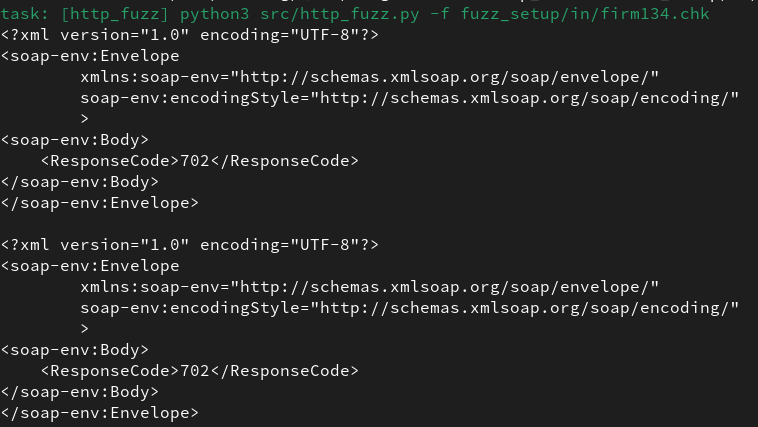
\includegraphics[scale=0.6]{SOAPfuzzing.png}
    \caption{Funcionamiento del script de fuzzing HTTP a UPNP.}
    \label{fig:SOAPfuzzing}
\end{figure}

\begin{figure}[H]
    \centering
    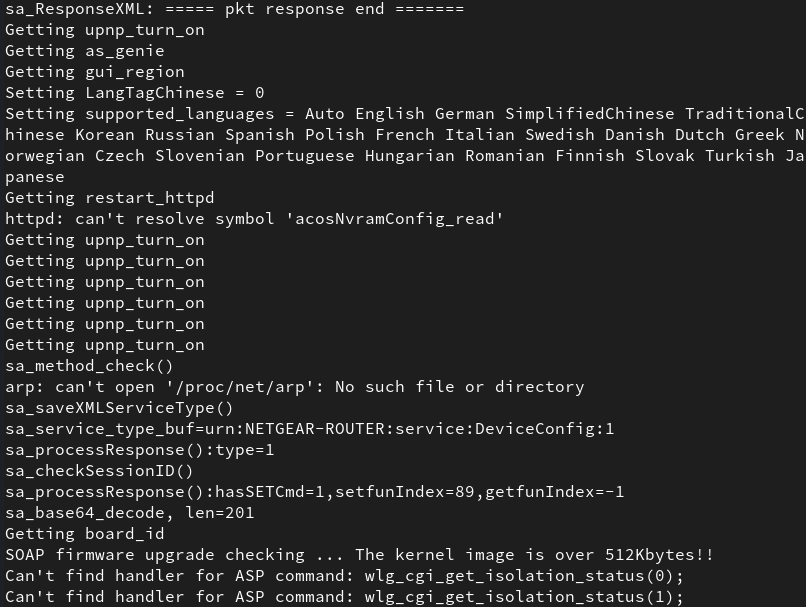
\includegraphics[scale=0.5]{SOAPprocessing.png}
    \caption{Servicio UPNP emulado procesando peticiones.}
    \label{fig:SOAPprocessing}
\end{figure}

\subsection{Resultados}
\subsubsection{Fuzzing con Qiling y AFL++}
Usar un script de Qiling con los bindings de python de Unicornafl para la integración con AFL++ ha resultado ser la opción menos efectiva. 
Aunque la parte de emulación se llevaba a cabo correctamente y con un gran incremento de velocidad gracias a tener que emular solo una función de 
código, tras las veinte horas y media de fuzzing no se detectó un solo crash ni timeout. Para analizar lo que estaba sucediendo, podemos hacer 
uso de la variable de entorno ''AFL\_DEBUG\_CHILD'' para ver el output del script en cada iteración de fuzzing. Haciendo esto, se detectaron dos 
problemas en la sesión de fuzzing causados por el mismo problema, uno a la hora de parsear los inputs del corpus y otro a la hora de mutarlos.\bigskip

Analizando el output de debugging se descubrió que Unicornafl, el componente de AFL++ que 
aporta la integración con Unicorn (y consecuentemente, Qiling) no gestiona correctamente los inputs que utilizan bytes nulos intercalados 
entre el resto de bytes. Esto provoca que por ejemplo, para las cabeceras de firmware que utilizamos como parte del corpus sus bytes sean 
tratados como una string de C y no como bytes, es decir, que a partir del primer byte nulo, el resto de bytes a continuación sean ignorados 
(figura \ref{fig:QilingDebug}). De esta forma, cuando AFL++ recibe un input para mutarlo, solo recibe los bytes de la primera sección 
de la cabecera TRX (la cadena mágica) y no es capaz 
de respetar la separación entre los campos de la cabecera mediante bytes nulos. Esto explica por qué no se ha obtenido ningún crash, ya que 
nunca se ha dado el caso de haber generado un input con la cadena mágica correcta delimitada por un byte nulo que además tuviera una valor 
excesivo en el siguiente campo del header para la longitud de este. Este problema ha sido discutido y reconocido por los principales 
desarrolladores del proyecto a través de Telegram y se ha dejado constancia a mediante la creación de un reporte a modo de issue en su repositorio
de \href{https://github.com/AFLplusplus/unicornafl/issues/13}{Github}. 
\begin{figure}[H]
    \centering
    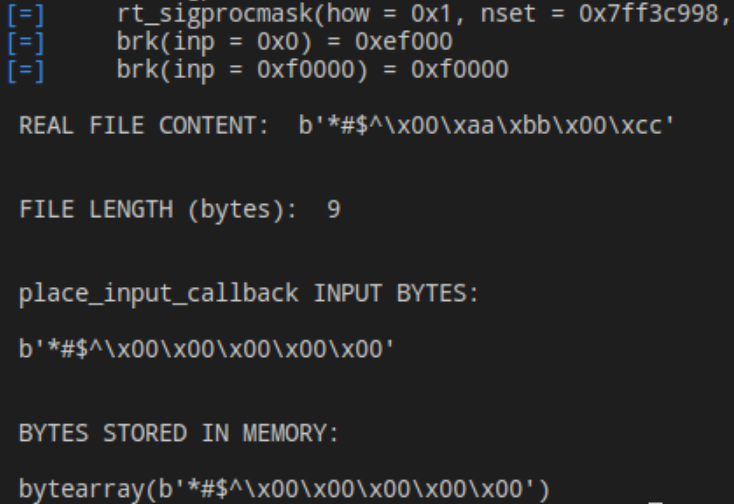
\includegraphics[scale=0.5]{QilingDebug.png}
    \caption{Mensajes de depuración en el script de Qiling mostrando la incorrecta gestión de inputs.}
    \label{fig:QilingDebug}
\end{figure}

Como solución temporal, podemos manualmente en el script de Qiling modificar el callback que almacena los inputs en memoria para fijar a 0
los bytes que actúen como delimitadores de las distintas secciones de una cabecera TRX. Por ejemplo, solo fijando a 0 el byte cuarto del input
(el que delimita la cadena mágica) ya podemos ver crashes en AFL++ en alrededor de un minuto (figura \ref{fig:QilingCheat}). Al analizar uno 
de los crashes generados (\ref{fig:UPNPQilingCrash}) apreciamos que efectivamente, AFL++ no ha introducido bytes nulos en el input para
separar las secciones y que si ha crasheado, ha sido por introducirlos manualmente desde el script previamente a almacenar los inputs en memoria.
En rojo los bytes que representan la cadena mágica, en verde el byte que será reemplazado a $\backslash$x00 como delimitador dentro del script y en
azul los bytes que indican el tamaño de la cabecera.

\begin{figure}[H]
    \centering
    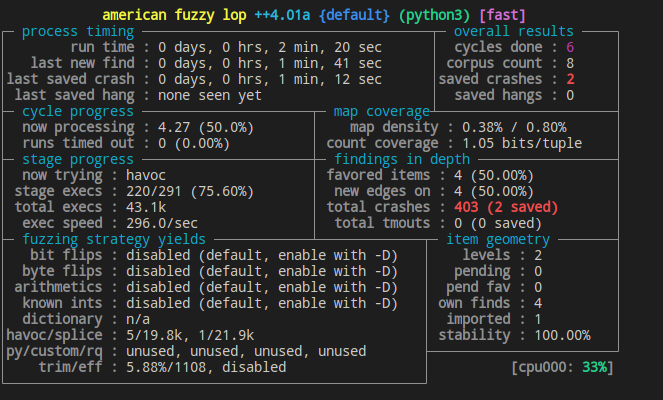
\includegraphics[scale=0.6]{QilingCheat.png}
    \caption{Fuzzing de UPNP con Qiling y AFL++ fijando manualmente el fin de la cadena mágica.}
    \label{fig:QilingCheat}
\end{figure}

\begin{figure}[H]
    \centering
    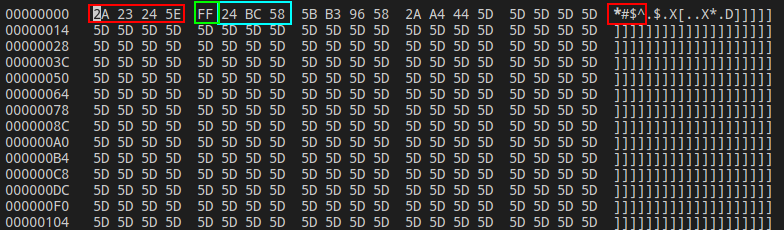
\includegraphics[scale=0.6]{UPNPQilingCrash.png}
    \caption{Cabecera firmware mutada por AFL++.}
    \label{fig:UPNPQilingCrash}
\end{figure}

Como hemos comentado, aunque la sesión de fuzzing no ha sido exitosa, Qiling ha dado muy buenos resultados a la hora de emular e instrumentar dinámicamente 
el binario. Es por ello que de estos resultados surge un pequeño experimento adicional. Esto es, integrar Radamsa con nuestro script de emulación de Qiling
para tener así un caso extra que nos permita comparar los resultados de fuzzear sobre emulación full-system en comparación con emulación basada en Unicorn 
manteniendo un mismo fuzzer. Respecto a las modificaciones del script, solo será necesario cambiar desde dónde obtiene el script el firmware por la misma
integración con Radamsa que hemos aplicado en el script de fuzzing a través de HTTP implementado anteriormente. Sorprendentemente, Radamsa
si que es capaz de identificar y respetar algunos de los campos presentes en las cabeceras, consiguiendo encontrar un crash en el binario
en aproximadamente 10 segundos haciendo uso del modo determinista y partiendo de la imagen firmware versión 1.0.11.134 (figura \ref{fig:UPNPQilingRadamsaCrash}).

\begin{figure}[H]
    \centering
    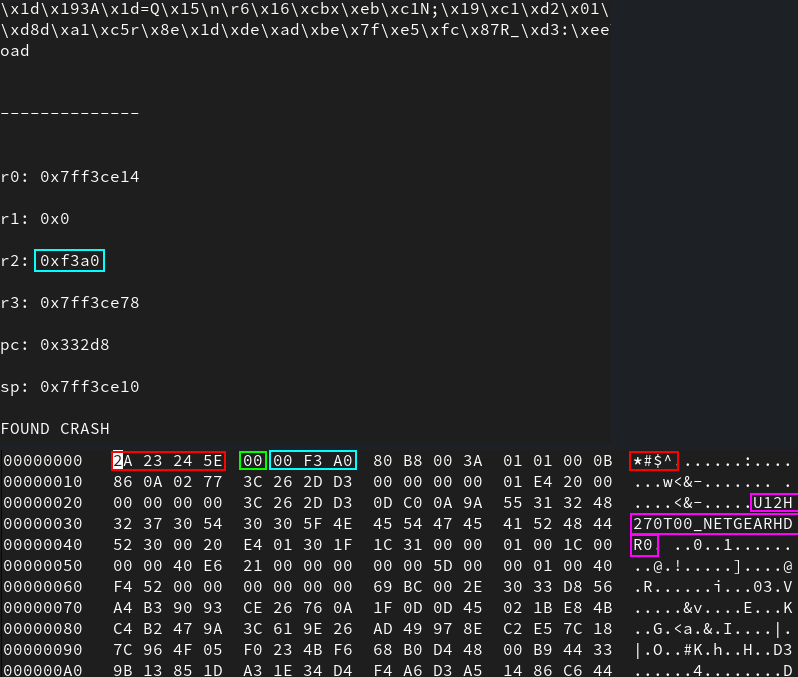
\includegraphics[scale=0.55]{UPNPQilingRadamsaCrash.png}
    \caption{Crash en UPNP identificado por Radamsa + Qiling.}
    \label{fig:UPNPQilingRadamsaCrash}
\end{figure}

\subsubsection{Fuzzing con QEMU full-system y Radamsa}
Al igual que Radamsa ha sido capaz de identificar el crash emulando el binario con Qiling en el caso anterior, también se ha llegado al mismo 
crash mediante el script desarrollado previamente que utiliza a Radamsa como fuzzer y va realizando peticiones SOAP a través de HTTP al 
demonio UPNP corriendo en la VM de QEMU ARM. La emulación tanto del sistema como del servicio ha sido estable durante todo el proceso de
fuzzing y UPNP era capaz de procesar correctamente las cabeceras del firmware enviado y de detectar si se producía algún fallo en la comprobación
de la cadena mágica o del checksum al igual que en Qiling. Para encontrar el mismo crash, partiendo de la misma semilla y funcionando en modo 
determinista, el script necesitó 1 minuto y 17 segundos (figura \ref{fig:UPNPQEMURadamsaCrash}), siendo el XML de la figura \ref{fig:UPNPQEMURadamsaCrashXML}
el causante del crash. Si comprobamos el estado del demonio en la VM (\ref{fig:UPNPsegfault}) observamos que como era de esperar, se ha producido un segmentation-fault
en la librería estándar de C (libc.so.0) mientras se realizaba la llamada a \textit{memcpy}.

\begin{figure}[H]
    \centering
    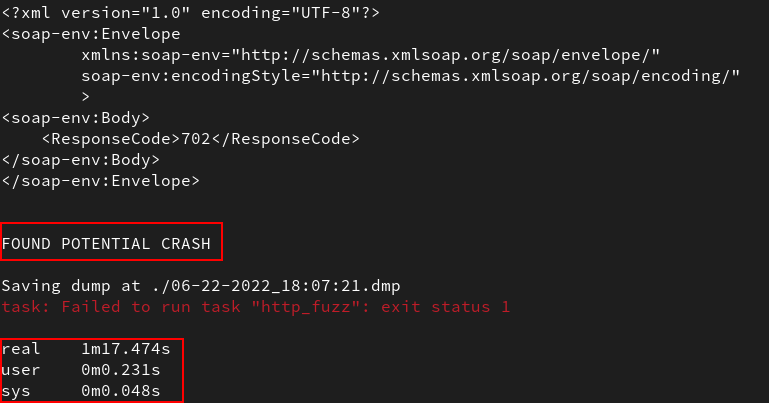
\includegraphics[scale=0.6]{UPNPQEMURadamsaCrash.png}
    \caption{Crash en UPNP identificado por Radamsa a través de peticiones HTTP.}
    \label{fig:UPNPQEMURadamsaCrash}
\end{figure}

\begin{figure}[H]
    \centering
    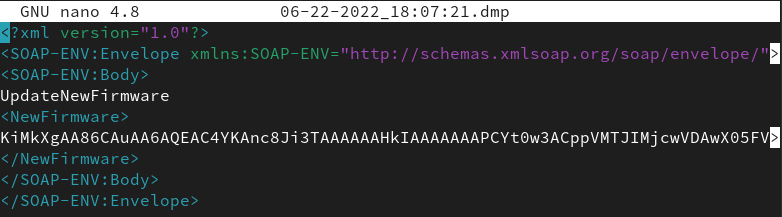
\includegraphics[scale=0.6]{UPNPQEMURadamsaCrashXML.png}
    \caption{Payload XML que ha causado el crash del servicio UPNP.}
    \label{fig:UPNPQEMURadamsaCrashXML}
\end{figure}

\begin{figure}[H]
    \centering
    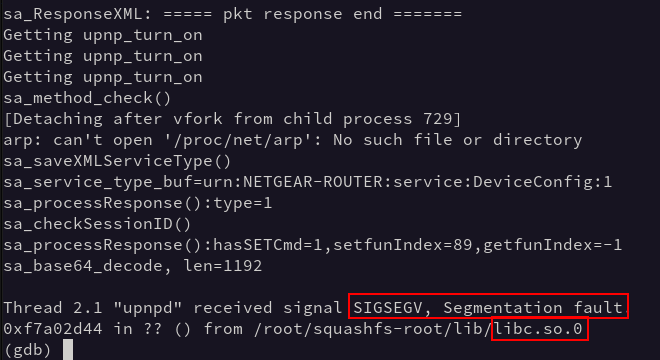
\includegraphics[scale=0.6]{UPNPsegfault.png}
    \caption{Segmentation-fault producido en UPNP durante el proceso de fuzzing HTTP.}
    \label{fig:UPNPsegfault}
\end{figure}

El gran incremento de tiempo para alcanzar la vulnerabilidad comparado con la aplicación de Radamsa junto a Qiling es comprensible, ya que 
no solo es necesario tener en cuenta el overhead de emular el sistema operativo al completo, sino que también las penalizaciones adicionales 
de rendimiento por emular el servicio al completo y por tener que enviar el firmware a través de peticiones HTTP.

\subsection{Lecciones aprendidas}
La realización de este experimento nos ha permitido sacar ciertas conclusiones respecto a la emulación y fuzzing de software orientado a IoT.
Principalmente podemos destacar los siguientes puntos:
\begin{itemize}
    \item Debido a que estamos ante una vulnerabilidad relativamente simple, hemos podido comprobar que hay casos para los que el uso de un 
    fuzzer de caja gris no aporta ninguna ventaja con respecto a aplicar fuzzing de caja negra. Obviando el bug de Unicornafl que hemos
    discutido, ambas técnicas han sido capaces de identificar la vulnerabilidad en periodos de tiempo similares.
    \item La integración de AFL++ con Unicorn/Qiling no está todavía lista para ser ampliamente adoptada por el público general. No es una 
    buena experiencia de usuario el no poder discernir si un problema encontrado durante el fuzzing es producido por un fallo personal 
    o por un fallo en la implementación de la herramienta.
    \item El uso del framework de Qiling resulta de gran utilidad cuando se quiere emular funcionalidad muy concreta de un binario y su 
    uso en combinación con otras herramientas de fuzzing facilita considerablemente el adaptar el binario al proceso de fuzzing gracias a 
    sus capacidades de instrumentación dinámica.
    \item Es recomendable depurar las sesiones de fuzzing para comprobar que el proceso se está realizando correctamente. En muchas ocasiones,
    es muy fácil cometer un error al realizar las preparaciones previas al fuzzing y es posible que aunque a primera vista el proceso se esté 
    llevando a cabo correctamente, realmente no se esté alcanzando el código que deseamos o no se estén identificando crashes que deberían de 
    ser registrados.
    \item La emulación full-system no nos permite prescindir completamente del hardware original, ya que como hemos podido comprobar, hay ciertos 
    casos para los que o se necesita extraer información del dispositivo original como variables de configuración o resulta difícil conseguir 
    emular a la perfección todos los periféricos requeridos.
\end{itemize}

\section{Análisis de un proyecto Open Source: Fuzzing de un parser JSON}
\subsection{Introducción al dispositivo}
La Wyzecam V3 (figura \ref{fig:wyzecam}) es una cámara de vigilancia WIFI de bajo coste fabricada por la empresa Wyze y lanzada al mercado
en 2020. Esta cámara representa
un claro ejemplo de dispositivo IoT, en el que toda la interacción con este se realiza a través de una app móvil además de disponer de integración con 
tecnologías comúnmente encontradas en domótica como Google Assistant, Amazon Alexa e IFTT.

\begin{figure}[H]
    \centering
    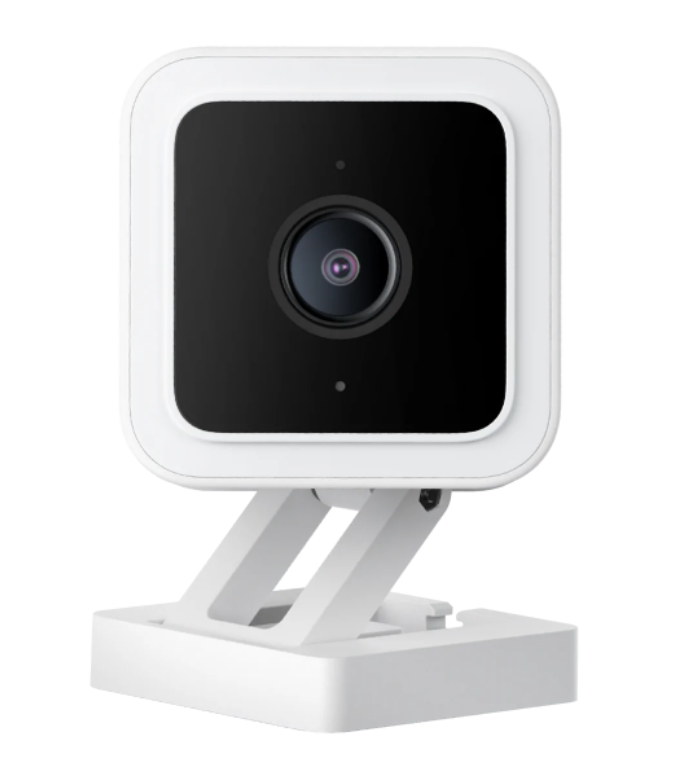
\includegraphics[scale=0.25]{wyzecam.png}
    \caption{Wyzecam V3.}
    \label{fig:wyzecam}
\end{figure}

\subsection{Recopilación de información}
Siguiendo el mismo procedimiento llevado a cabo en el apartado \ref{r7000_section} para obtener información más detallada sobre
el dispositivo, accedemos al reporte del FCC para la Wyzecam V3\cite{wyzecamFCCid} y a través de su listado de fotografías internas
identificamos su SoC. Rápidamente observamos que se trata de un ''Ingenic T31'' (figura \ref{fig:ingenict31}), un SoC orientado a procesamiento 
de vídeo. Consultando las especificaciones técnicas proporcionadas por el fabricante de este chip llegamos a un diagrama de bloques 
(figura \ref{fig:ingenicDiagram}) que nos indica que estamos ante un procesador modelo XBurst 1 con una arquitectura MIPS de 32 bits.
Para responder a la pregunta de si posee una MMU accedemos al manual de programación oficial del chip\cite{xburstmanual} y descubrimos 
que posee una MMU capaz de direccionar hasta 4GB de memoria.

\begin{figure}[H]
    \centering
    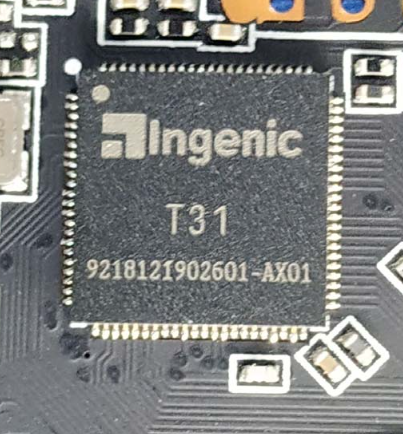
\includegraphics[scale=0.45]{ingenict31.png}
    \caption{SoC Ingenic T31 dentro de la Wyzecam V3\cite{wyzecamFCCid}.}
    \label{fig:ingenict31}
\end{figure}

\begin{figure}[H]
    \centering
    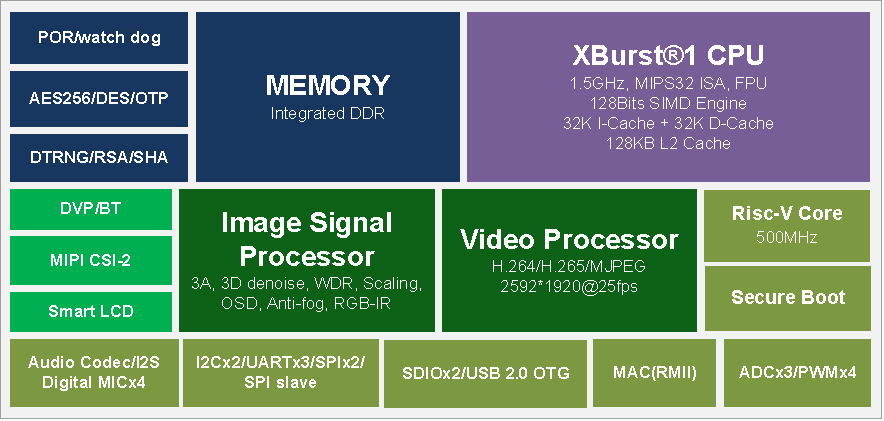
\includegraphics[scale=1.1]{ingenicDiagram.png}
    \caption{Diagrama de bloques del Ingenic T31\cite{ingenicproductpage}.}
    \label{fig:ingenicDiagram}
\end{figure}

\subsection{Obtención del firmware}
Para la obtención del firmware, accedemos al \href{https://support.wyze.com/hc/en-us/articles/360024852172-Release-Notes-Firmware}{portal de descargas}
de Wyze y descargamos la versión 4.36.8.26. El resultado es un fichero
con extensión ''.bin'' que procederemos a analizar con binwalk\cite{binwalk}. De la misma forma que anteriormente, empezamos consultando 
la entropía del firmware. Al hacerlo, como podemos observar en la figura \ref{fig:wyzeEntropy}, se muestra una entropía alta con caídas 
pronunciadas. Esto se debe a que el firmware está mayormente comprimido pero las cabeceras de sus secciones no lo están. Para comprobarlo,
utilizamos binwalk para obtener un reporte de los elementos contenidos dentro del binario y efectivamente, observamos que las caídas de 
la entropía dentro de los límites observables por binwalk se corresponden con la dirección de inicio de algunas de las secciones 
(figura \ref{fig:binwalkWyze}). También podemos ver que se utiliza un sistema de archivos SquashFS y que estamos ante un firmware basado
en Linux con un kernel versión 3.10.14 el cual fue publicado en 2013 y ha quedado ya considerablemente obsoleto. Por último, ya que se 
han detectado correctamente los contnidos del firmware, procedemos a su extracción para dar paso a la siguiente sección.

\begin{figure}[H]
    \centering
    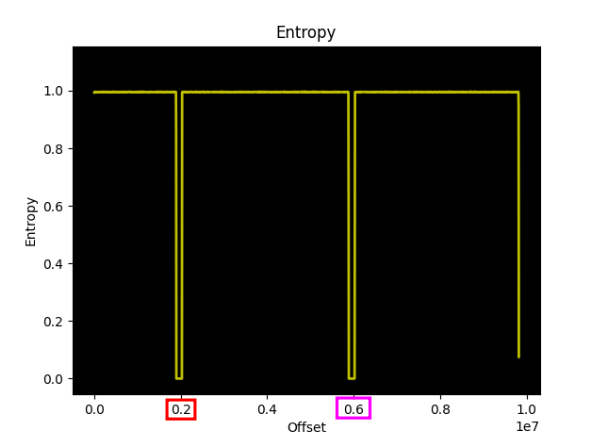
\includegraphics[scale=0.65]{wyzeEntropy.png}
    \caption{Entropía del firmware de la Wyzecam V3 versión 4.36.8.26.}
    \label{fig:wyzeEntropy}
\end{figure}

\begin{figure}[H]
    \centering
    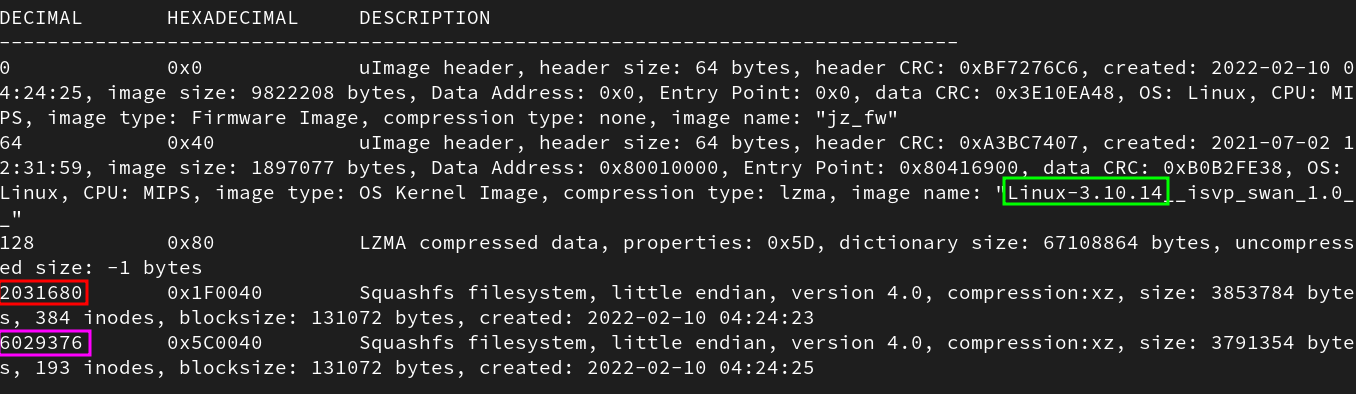
\includegraphics[scale=0.35]{binwalkWyze.png}
    \caption{Output de Binwalk sobre el firmware de la Wyzecam V3 versión 4.36.8.26.}
    \label{fig:binwalkWyze}
\end{figure}

\subsection{Introducción al experimento}
El componente software del firmware elegido para llevar a cabo este experimento es la librería cJSON, un parser de JSON extremadamente 
ligero escrito en ANSI C. Dado su bajo impacto en los recursos del sistema, esta librería es comúnmente usada en sistemas empotrados para
ayudar con el tratamiento de información en formato JSON. La motivación principal detrás de elegir este software para aplicar fuzzing es
la siguiente:
\begin{itemize}
    \item \textbf{Distribuida como librería}: El hecho de que cJSON esté incluido en el firmware a modo de librería enlazada dinámicamente y no como un ejecutable
    como sucedía en el anterior experimento, implica la necesidad de tratar un nuevo aspecto del fuzzing, los harness.
    \item \textbf{Superficie de ataque}: Los dispositivos IoT se caracterizan entre otras cosas por tratar con órdenes y datos provenientes del exterior
    desde de otros dispositivos. Para comunicar de forma eficiente esta información se suelen utilizar formatos como JSON o XML y por tanto, se 
    requerirán parsers que traten con esos inputs externos. Un fallo en el tratamiento de estos datos puede dar lugar a comportamientos erráticos o 
    presentar una oportunidad para un atacante.
    \item \textbf{Open Source}: Teniendo en cuenta que nos estamos introduciendo por primera vez en el campo del reversing y fuzzing en este tipo de 
    dispositivos, tener acceso al código fuente original puede ayudarnos a analizar más fácilmente los crashes encontrados y sus causas. Además, 
    aunque teniendo acceso al código fuente podríamos simplemente recompilarlo para x86-64, el centrarnos en trabajar con la librería extraída del firmware 
    nos da la oportunidad de seguir expandiendo nuestros conocimientos sobre este campo pero con la ayuda adicional de poder consultar el código original.
\end{itemize}

Habiendo tratado con el experimento anterior el uso de Qiling en profundidad y dado que en esta ocasión tenemos control sobre el harness a utilizar, centraremos
este experimento en el fuzzing de caja gris a través de AFL++ en modo QEMU. Además, comprobaremos si es posible obtener una mejora de resultados mediante 
el uso de desinfectantes como QASAN en conjunción con el proceso de fuzzing. Por último, cabe destacar que en este caso no partimos buscando una vulnerabilidad
ya conocida, sino que nuestro objetivo es intentar descubrir nuevas vulnerabilidades en el producto.

\subsection{Realización del experimento}
\subsubsection{Creación del harness}
Como hemos comentado, debido a que estamos tratando con una librería enlazada dinámicamente por distintos componentes del firmware del dispositivo, necesitaremos
implementar código a modo de harness que se encargue de obtener los inputs como parámetro de la línea de comandos y llame a ciertas funciones de la librería.
Para decidir qué funciones de la librería poner a prueba, un buen criterio a seguir es tratar aquellas funciones que trabajen directamente 
con input externo. Para conocer el listado de funciones de que exporta la librería hay dos posibles rutas a seguir. En primer lugar, si tenemos acceso al código
fuente como es el caso, podemos simplemente incluir el header file de la librería en nuestro harness. En caso de no tenerlo, es posible listar las funciones
exportadas por una librería compartida con herramientas como ''objdump'' o ''nm'' (figura \ref{fig:objdump}) y definir en nuestro harness las funciones usando 
la keyword de C ''extern'' para indicar al
compilador que la función será resuelta en tiempo de enlazado. Además, querremos que las funciones elegidas sean utilizadas por el firmware del dispositivo, lo
cual podemos comprobar desde el sistema de archivos extraído del firmware haciendo uso de un ''grep'' recursivo para ver qué binarios importan la librería y usando la herramienta ''strings'' para listar
las funciones de cJSON utilizadas por el binario (en caso de que el binario no haya sido strippeado) (figura \ref{fig:cJSONimports}).

\begin{figure}[H]
    \centering
    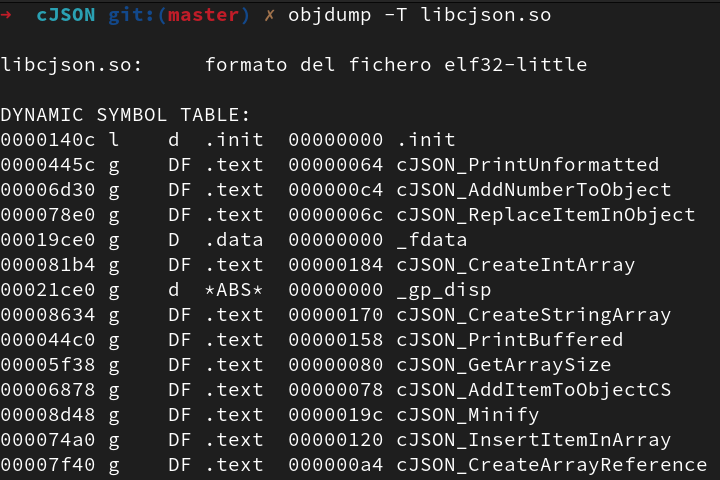
\includegraphics[scale=0.5]{objdump.png}
    \caption{Listado de las funciones exportadas por la librería de cJSON.}
    \label{fig:objdump}
\end{figure}

\begin{figure}[H]
    \centering
    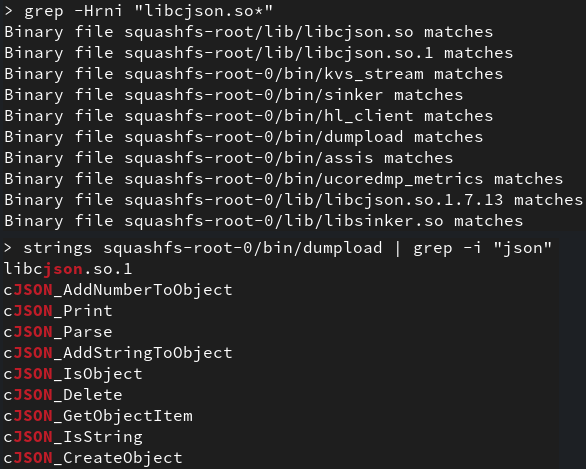
\includegraphics[scale=0.55]{cJSONimports.png}
    \caption{Listado de las funciones de la librería siendo utilizadas para un binario.}
    \label{fig:cJSONimports}
\end{figure}

Teniendo todo esto en cuenta, optamos por añadir al harness las siguientes funciones:
\begin{itemize}
    \item \textbf{cJSON\_Parse()}: Función principal encargada de parsear strings para generar una estructura de datos fácilmente manipulable que represente
    información en formato JSON. 
    \item \textbf{cJSON\_Minify()}: Función encargada de eliminar tokens innecesarios como saltos de línea de un input. 
    \item \textbf{cJSON\_Print()}: Función que imprime por pantalla el JSON parseado.
    \item \textbf{cJSON\_PrintBuffered()}: Alternativa a ''cJSON\_Print()'' que utiliza memoria dinámica.
\end{itemize}

Para la lectura de los inputs a partir de un fichero, implementamos la siguiente función que volcará el contenido del fichero en un array de bytes al que se le 
añadirá un byte nulo al final para indicar el fin del input y evitar así problemas con el tratamiento de los bytes en caso de que AFL++ genere una string mutada 
que no haya sido correctamente terminada.

\begin{lstlisting}[language=C, caption=Lectura de inputs desde fichero en el harness., captionpos=b,
    frame=single, breaklines, showstringspaces=false]
    char* read_input(char* path){
        FILE *f;
        struct stat st;
        char* content = NULL;
        size_t read_elements = 0;
    
        f = fopen(path, "rb");
        if (f == NULL)
            exit(1);
    
        stat(path, &st);
        if (st.st_size == 0)
            exit(1);
    
        content = (char*)malloc(st.st_size + 1);
        content[st.st_size] = '\0';                                                 // Avoid heap-buffer-overflow in strlen with non null terminated strings
        if (fread(content, st.st_size, 1, f) != 1 || strlen(content) == 0)
            exit(1);
        
        return content;
    }
\end{lstlisting}

Por último, compilamos el harness para MIPS indicándole al compilador que haga uso de la librería compartida de cJSON. Usaremos la 
siguiente orden con el compilador GCC de la toolchain de GNU para MIPS(el) y lo emulamos usando QEMU (figura \ref{fig:harnessRun}):

\begin{lstlisting}[language=bash]
    $ mipsel-linux-gnu-gcc -Iinclude src/harness.c -o bin/harness -lc -lcjson
\end{lstlisting}

\begin{figure}[H]
    \centering
    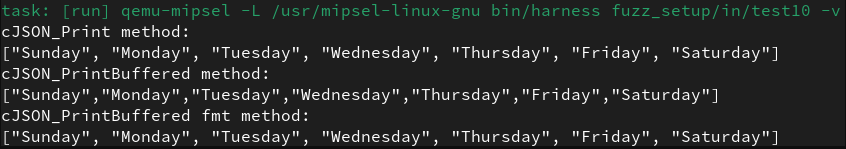
\includegraphics[scale=0.6]{harnessRun.png}
    \caption{Ejecución del harness en QEMU.}
    \label{fig:harnessRun}
\end{figure}

\subsubsection{Fuzzing de cJSON}
Comenzar la sesión de fuzzing con AFL++ en modo QEMU en sencillo, simplemente creamos un corpus de inputs 
con una serie de ficheros con datos en formato JSON e iniciamos AFL++ en modo QEMU (figura \ref{fig:harnessFuzz})
de la misma forma que se ha realizado en experimentos anteriores pero esta vez indicando con la variable de entorno
''AFL\_INST\_LIBS'' que deseamos que se instrumente también la ejecución de código en las librerías compartidas.

\begin{figure}[H]
    \centering
    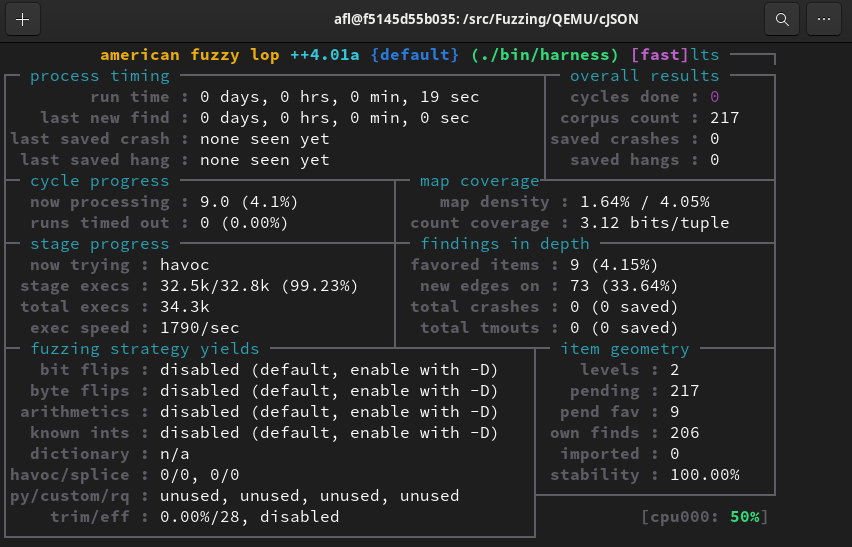
\includegraphics[scale=0.5]{harnessFuzz.png}
    \caption{Fuzzing del harness con AFL++ en modo QEMU.}
    \label{fig:harnessFuzz}
\end{figure}

AFL++ permite activar el uso de desinfectantes en su modo QEMU utilizando la variable de entorno ''AFL\_USE\_QASAN''.
QASAN hará uso de las capacidades de instrumentación dinámica internas de QEMU para monitorizar operaciones de memoria 
en binarios que no han sido instrumentados estáticamente y forzar un crash en caso de detectar fallos de memoria. 
Sorprendentemente, al fijar esta variable de entorno AFL++ no era capaz de iniciar la sesión de fuzzing indicando que 
todas las ejecuciones realizadas con los inputs iniciales del corpus habían crasheado, como podemos 
observar en la figura \ref{fig:aflQASAN}

\begin{figure}[H]
    \centering
    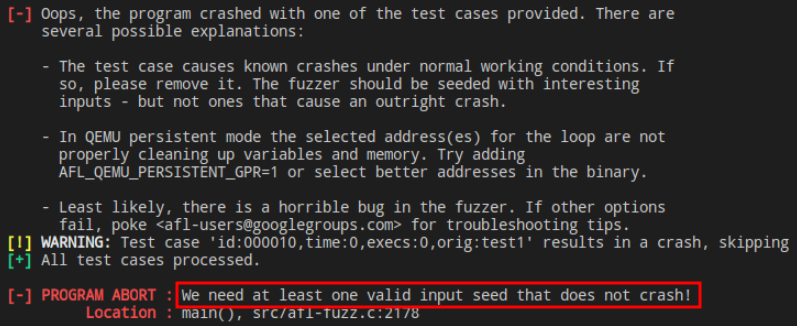
\includegraphics[scale=0.5]{aflQASAN.png}
    \caption{Error mostrado por AFL++ al activar QASAN para fuzzear cJSON.}
    \label{fig:aflQASAN}
\end{figure}

\subsection{Resultados}

- Alto uso de disco
- Falsos positivos (MIPS y por el harness)
- Confusión por QASAN
- Comparación de resultados con QASAN y AFL++

Durante la realización de este experimento, fue necesario hacer frente a una serie de problemas encontrados:
\begin{itemize}
    \item \textbf{Alto uso de I/O}: Cuando se realizar fuzzing, un factor que hemos de tener en cuenta es la carga 
    de I/O a la que el disco del host es sometido. En este experimento concretamente, el gran número de ejecuciones por 
    segundo y por tanto de escrituras de nuevos ficheros con inputs JSON mutados daba lugar a unos 7MB/s de escritura en 
    disco como podíamos comprobar con la herramienta ''iotop'' (figura \ref{fig:iotopBefore}). Mantener estas cifras de forma 
    prolongada durante horas puede suponer un desgaste considerable para el disco pero esto puede ser paliado haciendo uso 
    de un ramdisk. Un ramdisk no es más que asignar una sección de la RAM de un dispositivo para que actúe como si de un disco
    de almacenamiento se tratara. Para usar un ramdisk con AFL++ solo deberemos de crear un directorio en ''/dev/shm'' y usar la 
    variable de entorno ''AFL\_TMPDIR'' al iniciar la sesión de fuzzing para indicar que se desea utilizar el directorio creado para 
    la gestión de ficheros temporales durante el fuzzing. Este directorio especial se trata de un sistema de archivos temporal (tmpfs)
    encontrado en GNU/Linux que implementa el concepto de memoria compartida, utilizando RAM como medio de almacenamiento. Con este 
    cambio se consigue una reducción de escrituras en disco destacable, estando ahora ligeramente por encima de los 10KB/s 
    (figura \ref{fig:iotopAfter})
    \begin{figure}[H]
        \centering
        \includegraphics[scale=0.75]{iotopBefore.png}
        \caption{Uso de disco durante una sesión de fuzzing de cJSON.}
        \label{fig:iotopBefore}
    \end{figure}
    \begin{figure}[H]
        \centering
        \includegraphics[scale=0.54]{iotopAfter.png}
        \caption{Uso de disco tras utilizar un ramdisk durante una sesión de fuzzing de cJSON.}
        \label{fig:iotopAfter}
    \end{figure}
    \item \textbf{Aparición de falsos positivos}: 
    \item \textbf{Problemas para utilizar QASAN}

\end{itemize}

\subsection{Lecciones aprendidas}



